\documentclass[11pt, a4paper]{jreport}

\usepackage[driver=dvipdfm]{geometry}
\usepackage[dvipdfmx]{graphicx, color}
\usepackage{here}
\usepackage{plext}
\usepackage{times, mathptmx}
\usepackage{longtable}
\usepackage{colortbl}
\usepackage{tabularx}
\usepackage{enumerate}
\usepackage{comment}
\usepackage{url}
\usepackage{lscape}
\usepackage{multirow}
\usepackage{enumitem}
% code
\usepackage{minted}
\usepackage{mdframed}
% 
%\usepackage{otf}

\setlength{\voffset}{0.5truecm}
\setlength{\headsep}{2truecm}
\setlength{\oddsidemargin}{7.0truemm}
\setlength{\evensidemargin}{-5.5truemm}
\setlength{\topmargin}{-1truecm}
\setlength{\footskip}{25truemm}
\setlength{\textwidth}{15truecm}
\setlength{\textheight}{22truecm}
\renewcommand{\bibname}{参考文献}
\makeatletter
\makeatother

\begin{document}

\title{オープンソース開発プロセスの要素を導入した\\サーバ構築演習の授業設計と試験的評価\\Instructional Design and Evaluation of Server Exercise Class with Elements of Open Source Development Process}
\author{指導教員:深町 賢一\\
公立 千歳科学技術大学 理工学部\\
情報システム学科 深町研究室\\
令和4年度\\
B2190350 大森 裕介}
\date{\today}

\maketitle
\pagenumbering{roman}
\tableofcontents

\chapter{序論}
\pagenumbering{arabic}
\section{本研究の背景}

この章では,世界で求められているコンピテンシー教育と日本で行われている高等学校の情報教育,大学での実践的な情報教育について述べる.その後,これらの課題について述べる.

\subsection{コンピテンシー教育}\label{conpi}

文部科学省の資料によると,近年では図\ref{fig:oecd1}のような能力を教育機関でつけることが重要であると述べられている. 図\ref{fig:oecd1}には,各国のコンピテンシー教育と,経済協力開発機構(OECD)が述べるコンピテンシー教育について示されている\cite{bib:oecd}.

\begin{figure}[H]
\begin{center}
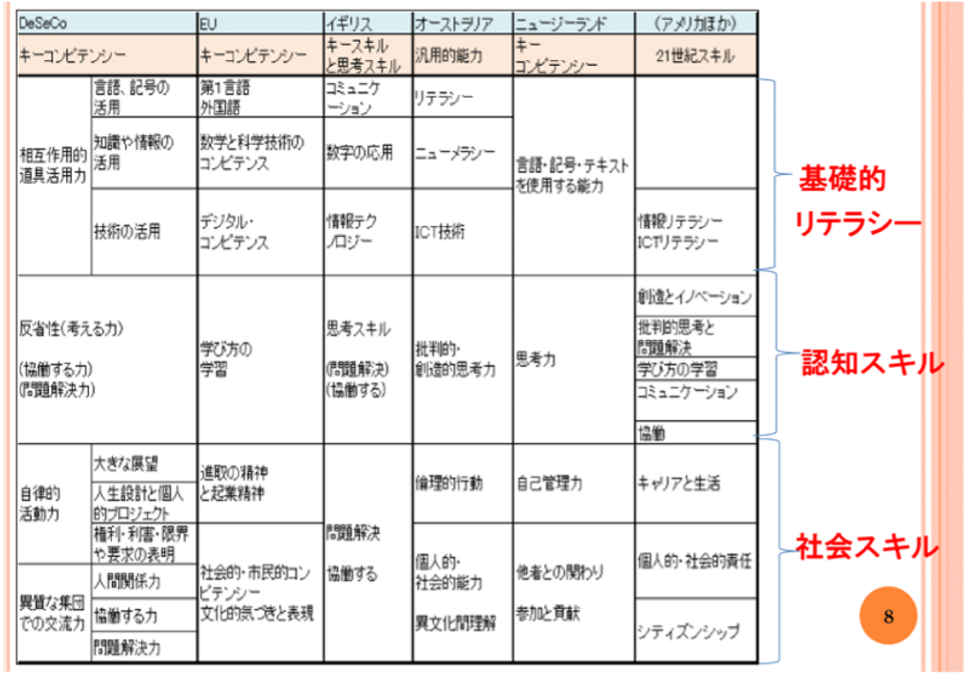
\includegraphics[width=140mm]{./img/oecd.png}
\caption{各国の目指すコンピテンシー教育(教育課程の編成に関する基礎的研究(P8)より引用)}
\label{fig:oecd1}
\end{center}
\end{figure}

OECDによると,基礎的リテラシーである相互作用的道具活用能力,認知スキルである反省性と社会スキルである自律的活動力,異質な集団での交流する能力を向上させることが必要であると述べられている.この中の反省力では,思考スキル,批判的思考,創造的思考が挙げられている.また,異質な集団での交流力では,異質な集団での問題解決が挙げられている.

経済産業省によると,「デジタルを活かすことで,場所,時間,年齢を問わず,誰であっても世界に広がる「本物」の社会課題に向き合い,探究学習を始められる環境が必要である」と述べられている\cite{bib:mirai}.決められた時間外にも多様な考え方を共有し,自ら学ぶことが必要である.多様な情報から探究学習を行うことは,OECDが示すコンピテンシー教育の項目と一致している.

\subsection{アクティブラーニング}\label{al_discription}

\ref{conpi}で述べた創造的思考の能力向上や学生の主体的な学習を促すためアクティブラーニングを取り入れた教育を行っている.文部科学省によりアクティブラーニングとは,「教員による一方向的な講義形式の教育とは異なり,学修者の能動的な学修への参加を取り入れた教授・学習法の総称である.文部科学省により,学修者が能動的に学修することによって,認知的,倫理的,社会的能力,教養,知識,経験を含めた汎用的能力の育成を図る.また,これらの能力育成のため,発見学習,問題解決学習,体験学習,調査学習等が含まれるが,教室内でのグループ・ディスカッション,ディベート,グループ・ワーク等も有効なアクティブ・ラーニングの方法である.」と定義されている\cite{bib:kyouikutennkann}.

\subsection{生涯学習}\label{shyougai}

学校教育を離れた人でも学び直しを行うことが求められている\cite{bib:shougai}.経済産業省によると,リカレント教育において,学問追求と実践的教育のバランスに留意しつつ,実践的な職業教育の拡充を図る必要がある.それと同時に,IT人材の育成も急がなければならないと述べられている\cite{bib:zinnzaikyouka}.

\subsection{日本の情報教育}\label{japan_zyouhou}

\subsubsection{高等学校情報科について}

令和4年度より,新しい高等学校学習指導要領に基づき,高等学校情報科においては共通必履修科目の情報Iが新設され,高等学校の全ての生徒がプログラミングやネットワーク,データベースの基礎について学習する\cite{bib:zyouhou}.大学教育では,発展的かつ実践的な教育を行う.

\subsubsection{情報処理技術者試験について}

基本情報技術者試験の資格取得を単位認定や入試優遇に用いている大学や授業カリキュラムを情報処理技術者試験の試験要綱を参考に策定している大学がある.大学教育のカリキュラムで情報処理技術者試験の試験要綱の知識を習得することが学生に求められている.

情報処理技術者試験とは,情報処理の促進に関する法律に基づき経済産業省が,情報処理技術者としての知識・技能が一定以上の水準であることを認定している国家試験である.情報処理技術者試験の試験要綱にはプログラミングやネットワーク,オープンソースソフトウェアなどについて出題されると示されている\cite{bib:kihonzyouhou_hani}.

\section{課題}\label{kadai_dai}

\ref{al_discription}で述べたアクティブラーニングにも課題がある.アクティブラーニングの課題を図\ref{fig:active_shippai}に示す.文部科学省によると,学生が安易な回答を求めることや派生知識に無関心,表面的な議論を行うこと,認知プロセスの外化(問題解決のために知識を使う,人に話す,書く,発表すること)を行わないことが課題だと述べている.これらの課題は,アクティブラーニングを行う前に学生に十分な知識がないことや,内発的モチベーションが低いことが原因であると述べられている\cite{bib:al_mondai}.

\begin{figure}[H]
\begin{center}
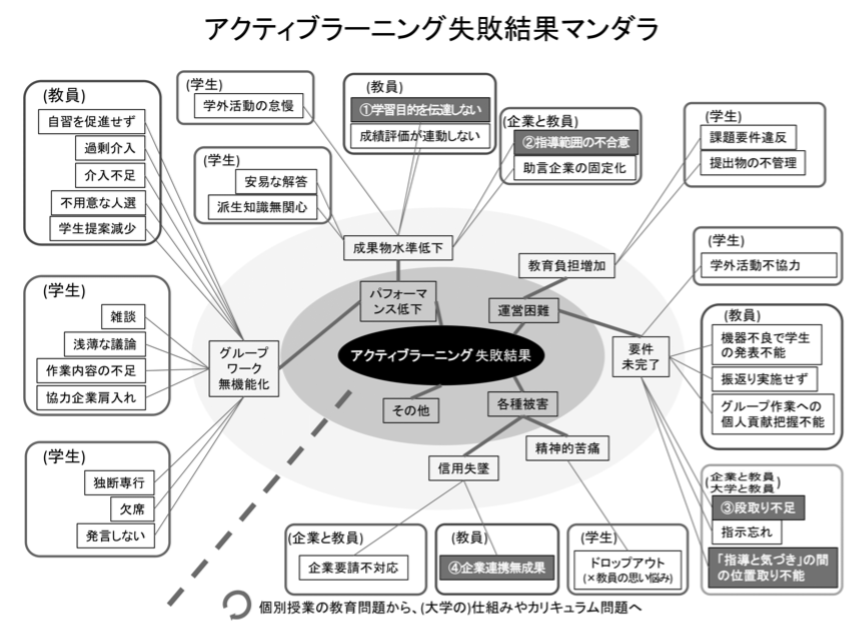
\includegraphics[width=140mm]{./img/al_mondai.png}
\caption{アクティブラーニング失敗結果マンダラ(「アクティブラーニング失敗事例ハンドブック~産業界ニーズ事業・成果報告~」(中部地域大学グループ・東海Aチーム、2014年(P3))より引用)}
\label{fig:active_shippai}
\end{center}
\end{figure}

\ref{shyougai}で述べた,生涯学習に主体的に取り組むためには,自身で情報の取捨選択を行い,情報の妥当性を調査する能力を身につける必要がある.

\ref{japan_zyouhou}で述べた,情報教育の進みにより,現在進みつつある社会構造の変動は,これまでになく大規模かつ急激なものである.大学教育では,発展的な情報教育を行う必要がある.教員には,これまで以上に高度な専門的知識・技能を修得し適時に刷新していくなど,教員に求められる資質能力の維持・向上を図るための更なる取組が必要とされている.しかし,教員は多くの業務を抱えており,教員に日々変化する高度な専門知識を習得させることは困難である\cite{bib:kyouinn_zituzyou}.

\section{本研究の目的}

近年,日本の教育では,積極的にIT技術者の育成を行っている.大学教育では,実践的な技術者育成も重要視されており,その技術者像や技術者教育の到達目標や評価方法の提言もされている.筆者は,発展的な知識や実践的な学習だけでなく,社会で求められるIT人材の開発姿勢や知識習得,実践的な能力を学ばせることも重要と考えている.姿勢や文化を学ぶ要素を授業設計に取り入れた場合の利点や欠点,また運用上の困難さについては明らかにされていない.

本研究では,オペレーティングシステムの仕組みについて学ぶ授業に,\ref{al_discription}で述べたアクティブラーニングに加え,オープンソースソフトウェア開発プロセスの要素である以下の要素を導入し,その有用性を評価する.

\begin{enumerate}[label=\textbf{(\alph*)}]
\item 非同期なコミュニケーション
\item 知識の集約,共有
\item 情報の妥当性を評価
\item 認知プロセスの外化
\item 異質な集団でのコミュニケーション
\end{enumerate}

\ref{conpi}で述べた異質な集団での交流する能力,批判的思考の向上を目指す.演習授業を行い,\ref{japan_zyouhou}で述べた実践的な学習を行う.\ref{shyougai}で述べたように,実践的な演習の中でオープンソースソフトウェア開発プロセスを実践し,教育機関を離れた後も主体的に学習できるIT技師術者を目指す学生に対する教育モデルの提案を行う.オープンソースソフトウェア開発プロセスの要素を取り入れた学習モデルはクラウドラーニング(Crowd learning)と呼ばれている\cite{bib:oss1} \cite{bib:oss2}.

オープンソースソフトウェアとオープンソースソフトウェア開発プロセス,クラウドラーニング,アクティブラーニングについての詳細は\ref{gakusyuumodel}で述べる.

\section{本論文の構成}

本論文は全5章で構成されている.2章では本研究で提案する学習モデルについて述べる.第3章では提案する学習モデルを本検証環境に適用する方法について述べる.第4章では検証結果について述べ,第5章で第4章で述べた結果から考察を行う.第6章では,第4章の結果や第5章の考察を踏まえ,今後の展望について述べる.

\chapter{学習モデル}\label{gakusyuumodel}

本章では本研究の基盤となる学習モデルであるオープンソースソフトウェア開発プロセス,オープンソースソフトウェアとクラウドラーニング(Crowd learning)について述べる.また,\ref{al_discription}で述べたアクティブラーニングの活用事例について述べる.その後,本研究で提案するアクティブラーニングにオープンソースソフトウェア開発プロセスの要素を取り入れた学習モデルについて述べる.

\section{オープンソースソフトウェア}\label{oss_discription}

ソースコードが公開されており,自由な利用,再配布を認めているソフトウェアがオープンソースソフトウェアと定義されている\cite{bib:oss_definition}.オープンソースソフトウェアの開発の多くは,無報酬で自発的に参加する開発者を中心として行われている.

\section{オープンソースソフトウェア開発プロセス}\label{osspr_discription}

オープンソースソフトウェア開発プロセスとは,オープンソースソフトウェア開発を行う過程である.オープンソースソフトウェア開発では,場所や時間にとらわれず,多様な考えや思考を行う人が協働しソフトウェアを開発している.そのため,テキストを主に用いてコミュニケーションを行っている.オープンソースソフトウェア開発に貢献する開発者は,知識をオープンソース開発から習得することや, オープンソースソフトウェア活動に貢献するため,自身の知識をオープンソースソフトウェア開発に提供する.しかし,提供される情報はさまざまで,情報の妥当性を多様な意見を交わしながら議論し,評価しながら開発を行う.

\section{クラウドラーニング(Crowd learning)}\label{cl_discription}

クラウドラーニングとは,オープンソースソフトウェア開発プロセスの概念を取り入れた学習モデルである\cite{bib:oss1}.学習者はインターネットなどの膨大かつ多様な情報源から情報を取得し,自身で妥当性を考察しながら学習する.インターネットの情報から学ぶことで,最新の専門知識の習得を行うことができるとされている.David Elijah Kaliszによると,「好きなときに好きな場所で学習できる機会が増えるにつれ,群衆学習を管理することがより複雑になる.学生をより自立させ,自分の学習経路(およびプロセス)を管理できるようにすることは、大きな利益をもたらす可能性がある.」と述べられている\cite{bib:oss2}.学生が自立し学習できるように促すことがクラウドラーニングでは重要である.また,学生自身で学習経路を管理することも必要である.

\section{アクティブラーニングの実例}

\subsection{金沢工業大学}

金沢工業大学では,「知識・スキルを取り込む」「様々な角度から考え、推論し、創造する」「修得した内容を発表、表現、伝達する」「総合的に評価を受ける」という過程を,すべての授業で導入し「考える力」「行動する力」を身につけることができるようなカリキュラムを作成し,実践している\cite{bib:kit}.

\subsection{広尾学園}

広尾学園の授業では,生徒はグループに分かれて自分たちで設定した研究テーマについて考察し,作成した資料をChromebookを用いて発表する.また,授業時間外では,ChromebookからGoogle Appsにアクセスすることで,生徒はどこにいても教員から資料や論文の内容についての指導が受けられる体制を整えている.この取り組みにより,学生が情報の集め方やその信憑性の把握などの研究テーマにアプローチする方法を学ぶ機会を作っている.また,研究活動では,ICTを活用したインターネットでの検索が不可欠であるが,ウェブ上にあふれる情報は答えでなく,考えるための材料であると述べられている\cite{bib:kitao}.

\section{本研究で提案する学習モデル}\label{gakusyuumoderu_base}

\subsection{オープンソースソフトウェア開発プロセスとクラウドラーニングの要素}

オープンソースソフトウェア開発プロセスとクラウドラーニング(Crowd learning)の要素を導入した学習モデルを提案する.本研究では,実践的な学習を行いながら,社会で求められるIT人材を意識させるためIT業界やオープンソースソフトウェア開発活動で用いられているGitHub\cite{bib:github}を利用し,次の学習姿勢の習得を促す.実践的な学習は\ref{gakusyuunaiyou}で述べる.

\begin{enumerate}[label=\textbf{(\alph*)}]
\item 時間や場所にとらわれない情報共有
\item 問題の発見から解決までの履歴を残す
\item 問題解決までの学習経路の把握
\item 異質な集団に近い状態でのコミュニケーション
\item 認知プロセスの外化(外部に発表)
\end{enumerate}

図\ref{fig:chisikimap}に学生間で情報共有し,整理された情報から学習経路を把握する様子を示す.GitHubを利用したコミュニケーションは必然的にテキストベースになる.GitHubを用いているため,時間や場所に関わらずコミュニケーションを行うことができる.テキストコミュニケーションでは情報や知識をまとめることが求められる.これにより言語リテラシー能力の必要性を理解させる.オープンソースソフトウェア開発活動のように匿名の状態で学生間のコミュニケーションを行い,異質な集団に近い状態でのコミュニケーションを行うようにする.他者からの情報は妥当性を評価し,表面的な議論を行いにくい状態を作る.学生全員に,GitHubで他者に貢献するように促した.また,貢献に対して評価し有益だと思う情報にはコメントを行ったりや,GitHubのスタンプ機能を用いて評価するように促した.

\begin{figure}[H]
\begin{center}
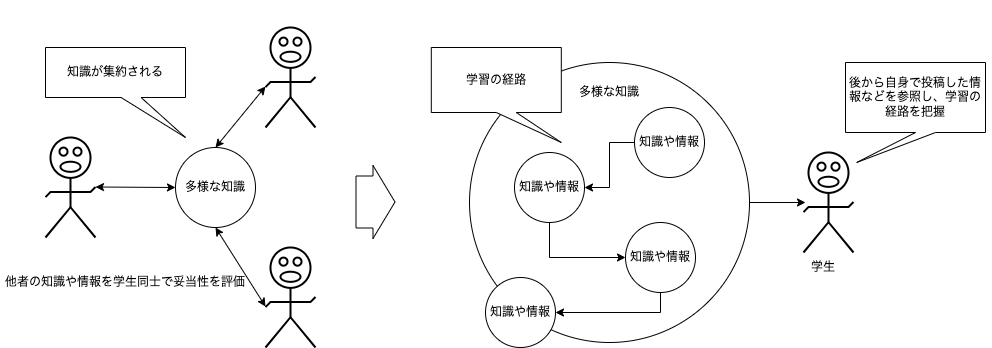
\includegraphics[width=140mm]{./img/chisikimap.png}
\caption{学生間で情報共有し,整理された情報から学習経路を把握}
\label{fig:chisikimap}
\end{center}
\end{figure}

知識の外化を促すため,習得した知識や情報の言語化が得意な学生には,その知識を課外活動で技術ブログを執筆することにより外部に公開することも促した.図\ref{fig:chisikiout}に技術ブログを執筆するために行う活動を示す.

習得した技術や知識を整理し,再度妥当性を評価する.技術ブログにするため,整理された情報を言語化する.その後,執筆した技術ブログを外部に公開し,外部の集団から閲覧,評価される.

\begin{figure}[H]
\begin{center}
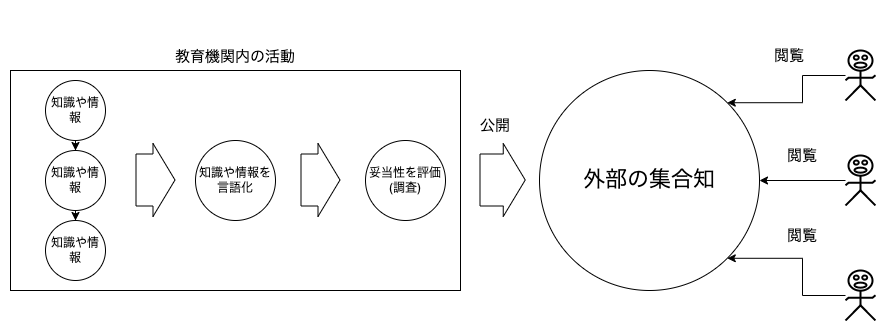
\includegraphics[width=120mm]{./img/gaibunikoukai.png}
\caption{知識を外部に公開}
\label{fig:chisikiout}
\end{center}
\end{figure}

\subsection{実践的な演習と興味,関心}\label{zissenn_kyoumi}

\ref{japan_zyouhou}で述べた実践的な学習も行う.実践的な学習の中で派生知識に関心を持つように促す.また,学生が学んだことがない知識や技術に触れさせることで,学生の興味や関心を促す.実践的な体験により学習意欲の向上を図る.授業時間外でも演習に取り組める環境を用意する.

\chapter{学習モデルの適用}

\section{本研究で提案する学習モデルを適用した授業設計}

本検証は全15回の演習授業で行った.授業構成は前半と後半で大きく分かれる.多くの学生はサーバ構築未経験者のため,前半では,テキストとワークシートを用いて,基本的なのアプリケーション構築を行い基礎から学習する.後半は「なんらかの連携をするシステムを構築する」という自由な課題とした.\ref{gakusyuumoderu_base}で述べた活動を促すためGitHubを用いたコミュニケーションを演習全体を通して利用する.

\subsection{学習者}

本学の情報システム工学科の学部3年の選択科目であるオペレーティングシステムを受講した学生である.学生は,本講義のE-learningで基本情報技術者試験で出題されるオペレーティングシステムの分野と同等の内容を学習している.他の授業でデータベースやネットワークについても学習している.

\subsection{授業内容}\label{gakusyuunaiyou}

\ref{gakusyuumoderu_base}で述べた学習モデルを本学の情報システム工学科の学部3年生の選択授業であるオペレーティングシステムの講義に導入し,検証を行った.

この演習は全てZoomを用いたオンライン授業形式で行った.オペレーティングシステムの講義は全15回の講義を行う.本検証の授業計画を以下の図\ref{tab:zyugyouplan}に授業計画を示す.

\begin{table}[!ht]
    \caption{全15回の授業計画}
    \label{tab:zyugyouplan}
    \centering
    \begin{tabular}{|l|l|l|l|l|}
    \hline
        授業回数 & 第1回 & 第2回〜第6回 & 第7回 & 第8回 \\ \hline
        授業形態 & オンライン & オンライン & オンライン & オンライン \\ \hline
        内容 & \begin{tabular}{c}調べ学習\end{tabular} & \begin{tabular}{c}LAMP環境\\構築演習\end{tabular} & \begin{tabular}{c}LAMP環境\\構築演習の\\口頭試問\end{tabular} & \begin{tabular}{c}E-learningの\\テスト\end{tabular} \\ \hline
        授業外学習 & E-learning & E-learning  & E-learning & 指示なし \\ \hline
        
        授業回数 & 第9回〜第14回 & 第15回 & \multicolumn{2}{|c|}{} \\ \hline
        授業形態 & オンライン & 対面 & \multicolumn{2}{|c|}{} \\ \hline
        内容 & \begin{tabular}{c}自由課題\end{tabular} & \begin{tabular}{c}自由課題の\\成果発表\end{tabular} & \multicolumn{2}{|c|}{}\\ \hline
        授業外学習 & 指示なし & 指示なし & \multicolumn{2}{|c|}{} \\ \hline
    \end{tabular}
\end{table}

前半の6回の演習授業では基礎的な学習を行う.講義時間外に,E-learningを用いて個人学習を行い,ネットワークやコンピュータの知識を学習する.演習授業時間では,実践的なサーバ構築演習を行う.この演習授業ではOSのLinux, WebサーバーのApache,データベースのMySQL,プログラミング言語のPHPを組み合わせた環境であるLAMPと呼ばれる環境をAmazon Web Services(AWS)\cite{bib:aws}が提供するEC2という仮想サーバ上に構築する.詳細は\ref{lamp_dis}で述べる.7回目の講義では,口頭試問を行い,学生が前半の演習内容を理解しながら演習を進めていたかについて調査した.

後半の9回目以降の演習では授業では,「なんらかの連携をするシステムを構築する」という自由な課題を提示し,個人やグループで課題を設定し,学生らで調査しながらサーバ構築を行うようにした.9回目以降の課題の成果物は15回目に学生全員の前で発表するようにした.

演習全体で時間や場所に関わらずAWSのサービスにアクセス可能な状態にし,いつでも演習に取り組めるようにした.GitHubも時間に関わらずコメントできるようにし,授業時間外もコミュニケーションが行える状態にした.

\subsubsection{LAMP構成のアプリケーション構築演習}\label{lamp_dis}

本学の他の講義では,WebアプリケーションをJavaを用いて作成する講義がある.そのため,アプリケーションの開発を通して,Webアプリケーションの仕組みについて実践的な経験を得て学んでいる.よって,学生がWebアプリケーションのプログラム部分については理解している.本検証では,最小限の機能しか持たないPHPで作成された簡単なプログラムのWebアプリケーション,データベース,WEBサーバを持つ基本的かつ最小構成であるLAMP環境を構築する.また,\ref{zissenn_kyoumi}で述べた学生の興味や関心を促すため,本学の学生は授業で学ばないPHPを選択した.

前半の6回の演習授業の内容についての詳細を表\ref{tab:ennsyuu_syousai}に示す.

\begin{table}[H]
\caption{LAMP構成のアプリケーション構築演習内容の詳細}
\label{tab:ennsyuu_syousai}
\centering
\begin{tabular}{|c|l|} \hline
授業回数 & \begin{tabular}{c}内容\end{tabular}\\ \hline
第1回 & \begin{tabular}{l}この回では,演習は行わず,第2回以降に用いるソフトウェア\\について学生自身でWeb検索を用いて調査することを行った.\end{tabular}\\ \hline
第2回 & \begin{tabular}{l}この回では,実践的な演習を行なった.\\仮想サーバであるEC2を作成し,\\作成したEC2に接続し,Apacheのインストールを行った.\end{tabular}\\ \hline
第3回 & \begin{tabular}{l}この回では,EC2にPHPをインストールし,\\ブラウザから動作していることを確認まで行った.\end{tabular}\\ \hline
第4回 & \begin{tabular}{l}この回では,EC2にデータベースであるMySQL\\をインストールし,データを追加する処理まで行った.\\また,正常にデータが保存されていることを確認した.\end{tabular}\\ \hline
第6回 & \begin{tabular}{l}この回では,第5回目での内容が完了している学生は,\\改良の余地が残されている\\LAMPのアプリケーションの改修を行った.\end{tabular}\\ \hline
\end{tabular}
\end{table}

学生は,表\ref{tab:ennsyuu_syousai}で示した演習で,図\ref{fig:phpapp}に示したアプリケーションを作成する.このアプリケーションはPHPで動作しており,テキストを入力することで,内容がデータベースに保存される.同様に,ボタンを押すことでデータをデータベースから削除することができる.複雑な機能を持たないアプリケーションにし,PHPのプログラムの理解に時間がかからないようにした.また,本演習の本質である,データベースとの接続やデータベースとのデータのやり取り,HTTPでのデータのやり取りの理解に注力できるようにした.

\begin{figure}[H]
\begin{center}
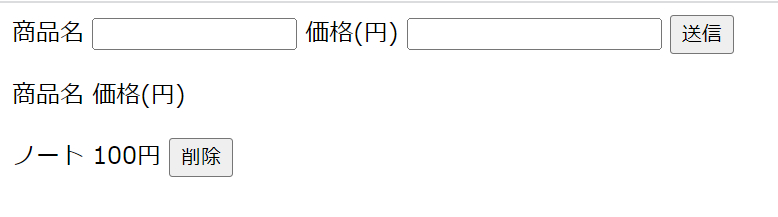
\includegraphics[width=120mm]{./img/phpapp.png}
\caption{本検証で学生が作成するアプリケーション}
\label{fig:phpapp}
\end{center}
\end{figure}

\subsubsection{後半の演習課題}

「なんらかの連携をするシステムを構築する」という自由な課題では,前半のLAMP構成のアプリケーション構築演習で学んでいないことに積極的に学び,サーバ構築演習に取り組むように促した.後半の課題でもEC2が利用できる状態にした.また,利用可能なAWSの他のサービスも紹介した.

\section{導入したアプリケーションや資料}

ここでは前半の演習授業であるLAMP構成のアプリケーションの構築演習で用いた資料やツールについて述べる.また,本検証全体を通して用いたコミュニケーションツールについても述べる.

\subsection{GitHub Issues}\label{GHIssue}

本検証では,文字でのコミュニケーションや思考の整理,文字で整理された思考を後から参照するためのツールとしてGitHubが提供するディスカッション機能のGitHub Issuesを採用した.GitHub Issuesはオープンソースソフトウェア開発でよく用いられており,知識の集約や,複数人での議論で用いられている.前述のアプリケーションを用いて時間や場所にとらわれずに世界中のエンジニアが議論しながらオープンソースソフトウェアの開発を行っている.

学生が,演習内で生じた問題を解決できなかった場合や演習内での疑問点や発見についてGitHub Issuesにコメントを投稿し,学生同士で議論しながら解決できるように用意した.図\ref{fig:issuelist}に本検証で用意したGitHub Issuesの様子を示す\cite{bib:ghissue}.自身の課題をタイトルにし,投稿する.学生らは,同様な課題のコメントを参照し,自身の演習環境に適用する.学生同士がお互いに認知しにくい状態でディスカッションすることで,情報の妥当性などを学生自身で考慮しながらコメントを読むことができる.

\begin{figure}[H]
\begin{center}
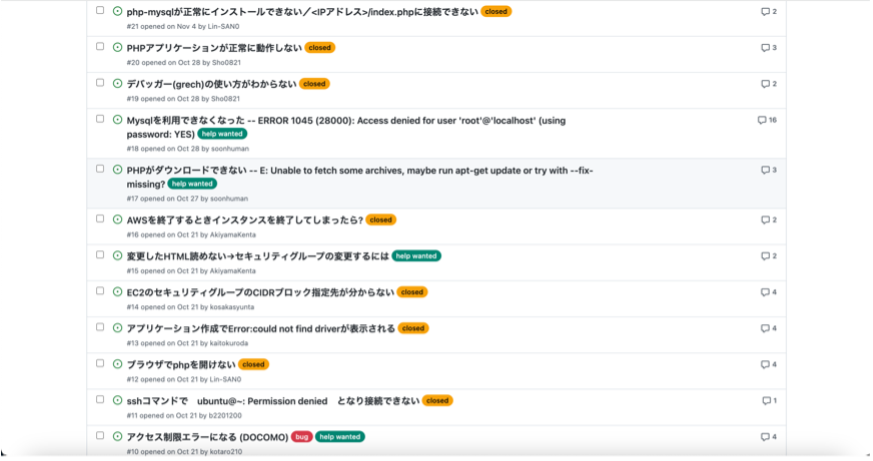
\includegraphics[width=140mm]{./img/issuelist.png}
\caption{GitHub Issuesでのコミュニケーションの様子}
\label{fig:issuelist}
\end{center}
\end{figure}

記載する内容は,以下のことについて書くように提示した.「何をしようとしているのか」「何故それがしたいのか」「エラーログ」「エラーの解決のために行ったこと」の4つの項目である.1つの問題についての会話の流れがスレッドに集約され,学習の流れを把握することができる.また,コメントを残すごとに調査,妥当性の評価,実践を行える.

\subsection{ワークシート,参考資料}

学生には,演習の内容を示すため,表\ref{tab:ennsyuu_syousai}で示した内容に沿ってワークシートを作成した.学生はワークシートに取り組みながら演習を行う.ワークシートでは演習に関することを幅広く設問にしている.サーバ構築を行うだけではなく,必要な動作の意味や仕組みを問う設問も用意した.

本演習に取り組む学生で,サーバ構築を経験している学生は少ないため,基礎知識の習得のため,ワークシートに準拠したサーバ構築演習の資料\cite{bib:lamp}を作成した.資料の一部を図\ref{fig:worksheet}に示す.資料では,派生知識に関する外部の資料の提示も行った.また,演習で用いたコマンドや知識を解説している.詳細については参考になるインターネット上の資料を明示しており,知識を学生自身で深められるようにしている.これにより,ワークシートを参考に演習に取り組み,不明点は資料を参照しながら理解を深められるようにした.

\begin{figure}[H]
\begin{center}
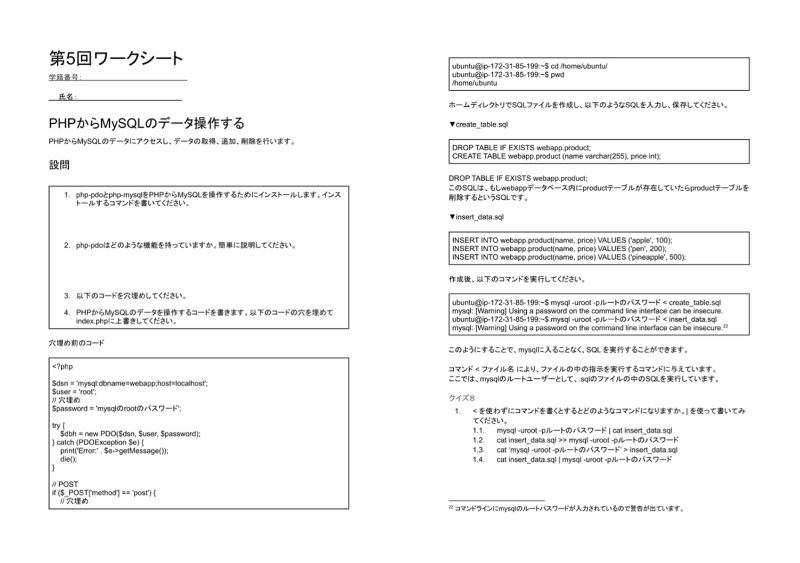
\includegraphics[width=120mm]{./img/worksheet.png}
\caption{(左)ワークシート,(右)参考資料}
\label{fig:worksheet}
\end{center}
\end{figure}

\subsection{サーバ構築演習支援ツール}\label{grech}

上記のワークシートや資料に加え,学生が課題や問題点を発見し,主体的に課題解決を促すため,調査を支援するためのツール\cite{bib:servertool}を開発した.本演習を行う学生は,サーバ構築の経験がない学生が多い.そのため,実践的な演習を行うには前提となるコマンドラインでの操作などの知識が不足している.そのため,前提知識や経験が浅い学生に対して,自身で問題を認知し,調査するための支援するための仕組みが必要だと考えた.このサーバ演習支援ツールでは,AWSのEC2内でツールを実行することができる.ツールによりどこに問題が存在しているのかを調査し,演習者に解決策や問題点を提示することができる.

\section{認知プロセスの外化}

前半のLAMP構成のアプリケーション構築演習終了後にLAMP構成の構築演習についての口頭試問を行った.後半の演習課題終了後に習得した知識や成果物についての発表を他の学生の前で発表を行った.また,後半の課題で取り組みたいことについて調査し,前半の演習後に他の学生の前で発表を行った.

知識を外部に発表する活動を授業内で学生に勧めた.具体的には,授業時間外で技術ブログを執筆することを勧めた.学生に,ブログの書き方やブログの内容の提案を行った.また,授業内では教育機関外の集団に知識を公開することは困難なため,ブログの執筆を学生に勧めた.執筆した学生には,執筆したブログをQiita Advent Calendar\cite{bib:qiita}に登録するように促し,Qiita Advent Calendarから他の学生もブログを閲覧できるように管理した.

\chapter{評価}\label{hyouka}

本研究では, LAMP環境構演習開始前と築演習後にアンケートを行った.このアンケート結果の評価を行う.また,演習期間内に投稿されたIssueについても評価を行う.

\section{ARCSモデルに関するアンケートの結果}

本検証を行う前と第6回講義後にアンケートを行った.同じような質問を2回行い,どのように変化したかを以下に示す.このアンケートではARCSモデルを参考に作成した.ARCSモデルとは, 注意(Attention),関連性(Relevance),自信(Confidence),満足感(Satisfaction)の4要素の頭文字をとった学習モデルである.この4要素が学習意欲を向上させる要因になると言われている\cite{bib:arcs}.
 
アンケートでは,本検証で用いた本研究で提案する学習モデルにより,学生の演習に対する満足度や自信が向上しているかを調査する.本研究で提案する学習モデルにおいても,学習者のARCSモデルの要素を向上させることは,主体的に学習を促すために不可欠であると考えたためである.

検証前では,満足感を調査することはできないため,「注意」「関連性」「自信」の3項目をアンケートにより調査した.上記の3項目についてのアンケートの質問項目を以下に示す.有効なアンケート回答数は25件である.ARCSモデルの上記に示した3項目の効果を測定するアンケート項目は以下に示す.回答はリッカート尺度に沿った6つの選択肢でそれぞれ作成した.

\subsection{注意に関する設問}

検証前のアンケートの質問内容「第1〜2回の説明を聞いてインフラ構築に興味を持ちましたか」,検証後のアンケートの質問内容「今までの演習を行い、インフラ構築に興味を持ちましたか」

\paragraph{回答項目}

「とても興味を持った」「興味を持った」「少し興味を持った」「あまり興味を持たなかった」「興味を持たなかった」「全く興味を持たなかった」

\subsection{関連性に関する設問}

検証前のアンケートの質問内容「第3回以降に取り組む演習について、あなた自身の経験は役立ちそうだと思いましたか。」,検証後のアンケートの質問内容「今までの演習は、あなた自身の経験は役立ちそうだと思いましたか。」

\paragraph{回答項目}

「とても思う」「思う」「少し思う」「あまり思わない」「思わない」「全く思わない」

\subsection{自信に関する設問}

検証前のアンケートの質問内容「自分で解決法を探して取り組むことに対し、できそうだと思いましたか。」,検証後のアンケートの質問内容「自分で解決法を探して取り組むことができましたか。」

\paragraph{回答項目}

「とても思う」「思う」「少し思う」「あまり思わない」「思わない」「全く思わない」

\subsection{インフラ構築に対しての興味(注意)}

表\ref{tab:kyoumi}にARCSモデルの「注意」の変化を示す.インフラ構築に対しての興味の変化に対する学生の人数と学生の割合を示す.

\begin{table}[H]
\caption{インフラ構築に対しての興味(注意)}
\label{tab:kyoumi}
\centering
\begin{tabular}{|c|c|c|} \hline
注意の変化 & 人数 & 割合\\ \hline
向上 & 9人 & 36\% \\ \hline
変化なし & 15人 & 60\% \\ \hline
低下 & 1人 & 4\% \\ \hline
\end{tabular}
\end{table}

\subsection{将来役に立つかどうかについて(関連性)}

表\ref{tab:yakudatu}にARCSモデルの「注意」の変化を示す.インフラ構築は将来役に立つかについての変化に対する学生の人数と学生の割合を示す.

\begin{table}[H]
\caption{将来役に立つかどうかについて(関連性)}
\label{tab:yakudatu}
\centering
\begin{tabular}{|c|c|c|} \hline
関連性の変化 & 人数 & 割合\\ \hline
向上 & 8人 & 32\% \\ \hline
変化なし & 10人 & 40\% \\ \hline
低下 & 7人 & 28\% \\ \hline
\end{tabular}
\end{table}

\subsection{自信があるかについて(自信)}

表\ref{tab:zisin}にARCSモデルの「自信」の変化を示す.演習内容のインフラ構築に自信があるかについての変化に対する学生の人数と学生の割合を示す.

\begin{table}[H]
\caption{演習内容のインフラ構築に自信があるかについて(自信)}
\label{tab:zisin}
\centering
\begin{tabular}{|c|c|c|} \hline
自信の変化 & 人数 & 割合\\ \hline
向上 & 13人 & 52\% \\ \hline
変化なし & 10人 & 40\% \\ \hline
低下 & 2人 & 8\% \\ \hline
\end{tabular}
\end{table}

\section{最終課題に関する結果} 

LAMP構成のアプリケーション構築演習終了後の授業後半(第6回目)以降の演習で,LAMP環境構築演習で学んでいない知識や教員が示した課題以外に取り組もうと考える学生の変化を表\ref{tab:saisyuu}に示す.

\begin{table}[H]
\caption{最終課題で自身で課題を設定し取り組みたいか}
\label{tab:saisyuu}
\centering
\begin{tabular}{|c|c|c|} \hline
 & 演習前 & 演習後\\ \hline
自身で課題を設定し構築 & 2人 & 12人 \\ \hline
提示された課題から課題を決定 & 23人 & 13人 \\ \hline
\end{tabular}
\end{table}

表\ref{tab:saisyuu}より,自身で課題を設定し構築したいと思う学生が演習前と比較し,演習後に増加した.教員が提示した課題に取り組みたいと思う学生は減少していることが分かる.

\section{グループワークとテキストコミュニケーションの結果}\label{gw_tc_diff}

LAMP環境構築のワークシートが順調に進んだと感じた学生と,順調に進まなかったと感じた学生に分けて集計した結果を以下に示す.この2つの区分は学生の自己申告である.第7回の授業に行ったアンケートの「ワークシートの演習は順調に進みましたか」の設問に対して,「順調に進んだ」と回答した学生は「ワークシートが順調に進んだ学生」とした.反対に,「Issueを使いながら進めた」「順調に進まなかった」と回答した学生は「ワークシートが順調に進まなかった学生」として集計した.アンケート回答者が25名に対して,「ワークシートが順調に進んだ学生」は9名,「ワークシートが順調に進まなかった学生」は16名だった.

本検証以外での講義で行われているアクティブラーニングでのグループワークでの発言に関する設問の「グループワークで積極的に他者の発言にコメントできたと思いますか」と,本検証でのGitHub Issuesで他者にコメントできたかに関する設問の「積極的に他者のIssueにコメントできたと思いますか」の結果をグラフで図\ref{fig:gh_vs_gw_yes}, 図\ref{fig:gh_vs_gw_not}に示した.図\ref{fig:gh_vs_gw_yes}のグラフは「ワークシートが順調に進んだ学生」の結果を示し,図\ref{fig:gh_vs_gw_not}の左のグラフは「ワークシートが順調に進まなかった学生」の結果を示す.
それぞれのグラフの縦軸は,グループワークで他者に対して積極的にコメントできたと感じているかについての回答をスコア化した値,GitHub Issuesで積極的に他者の問題にコメントできたかについての回答をスコア化した値を示している.横軸は学生ごとの回答を示している.

\begin{figure}[htbp]
  \begin{minipage}[c]{.5\linewidth}
    \centering
    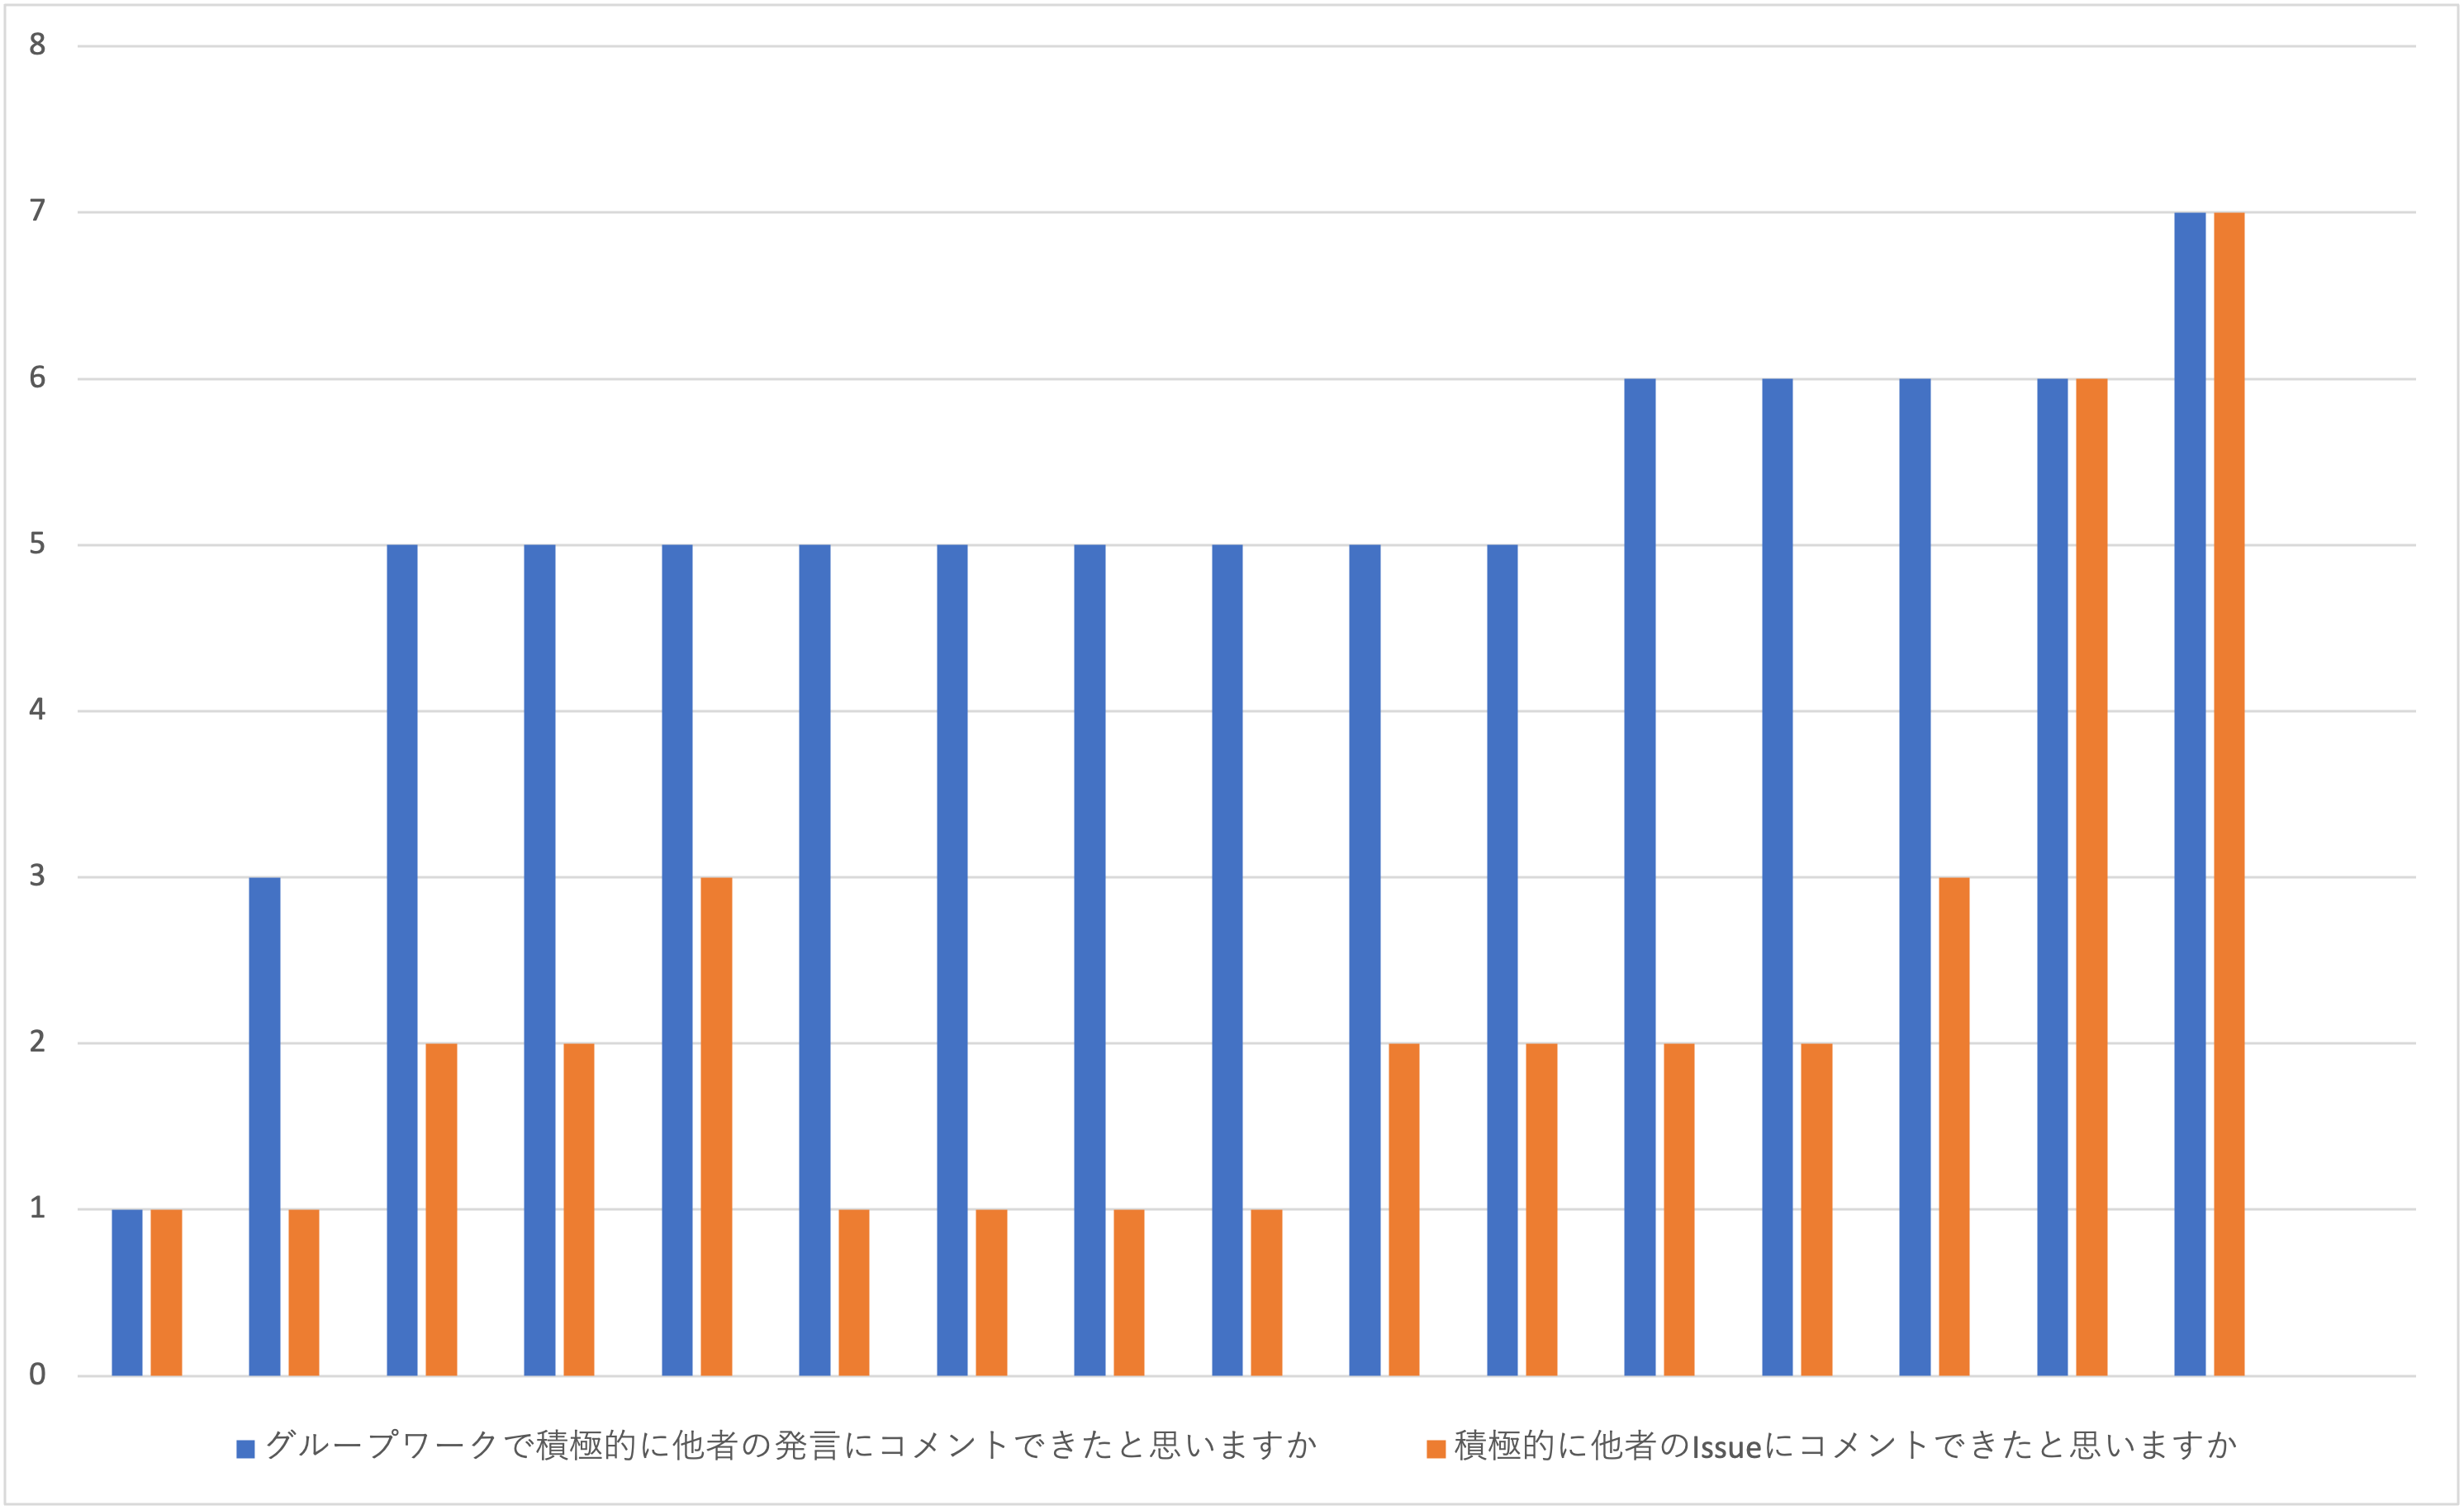
\includegraphics[width=1\linewidth]{img/gh_vs_gw_yes.png}
    \caption{ワークシートが順調に進んだ学生}
    \label{fig:gh_vs_gw_yes}
  \end{minipage}
  \begin{minipage}[c]{.5\linewidth}
    \centering
    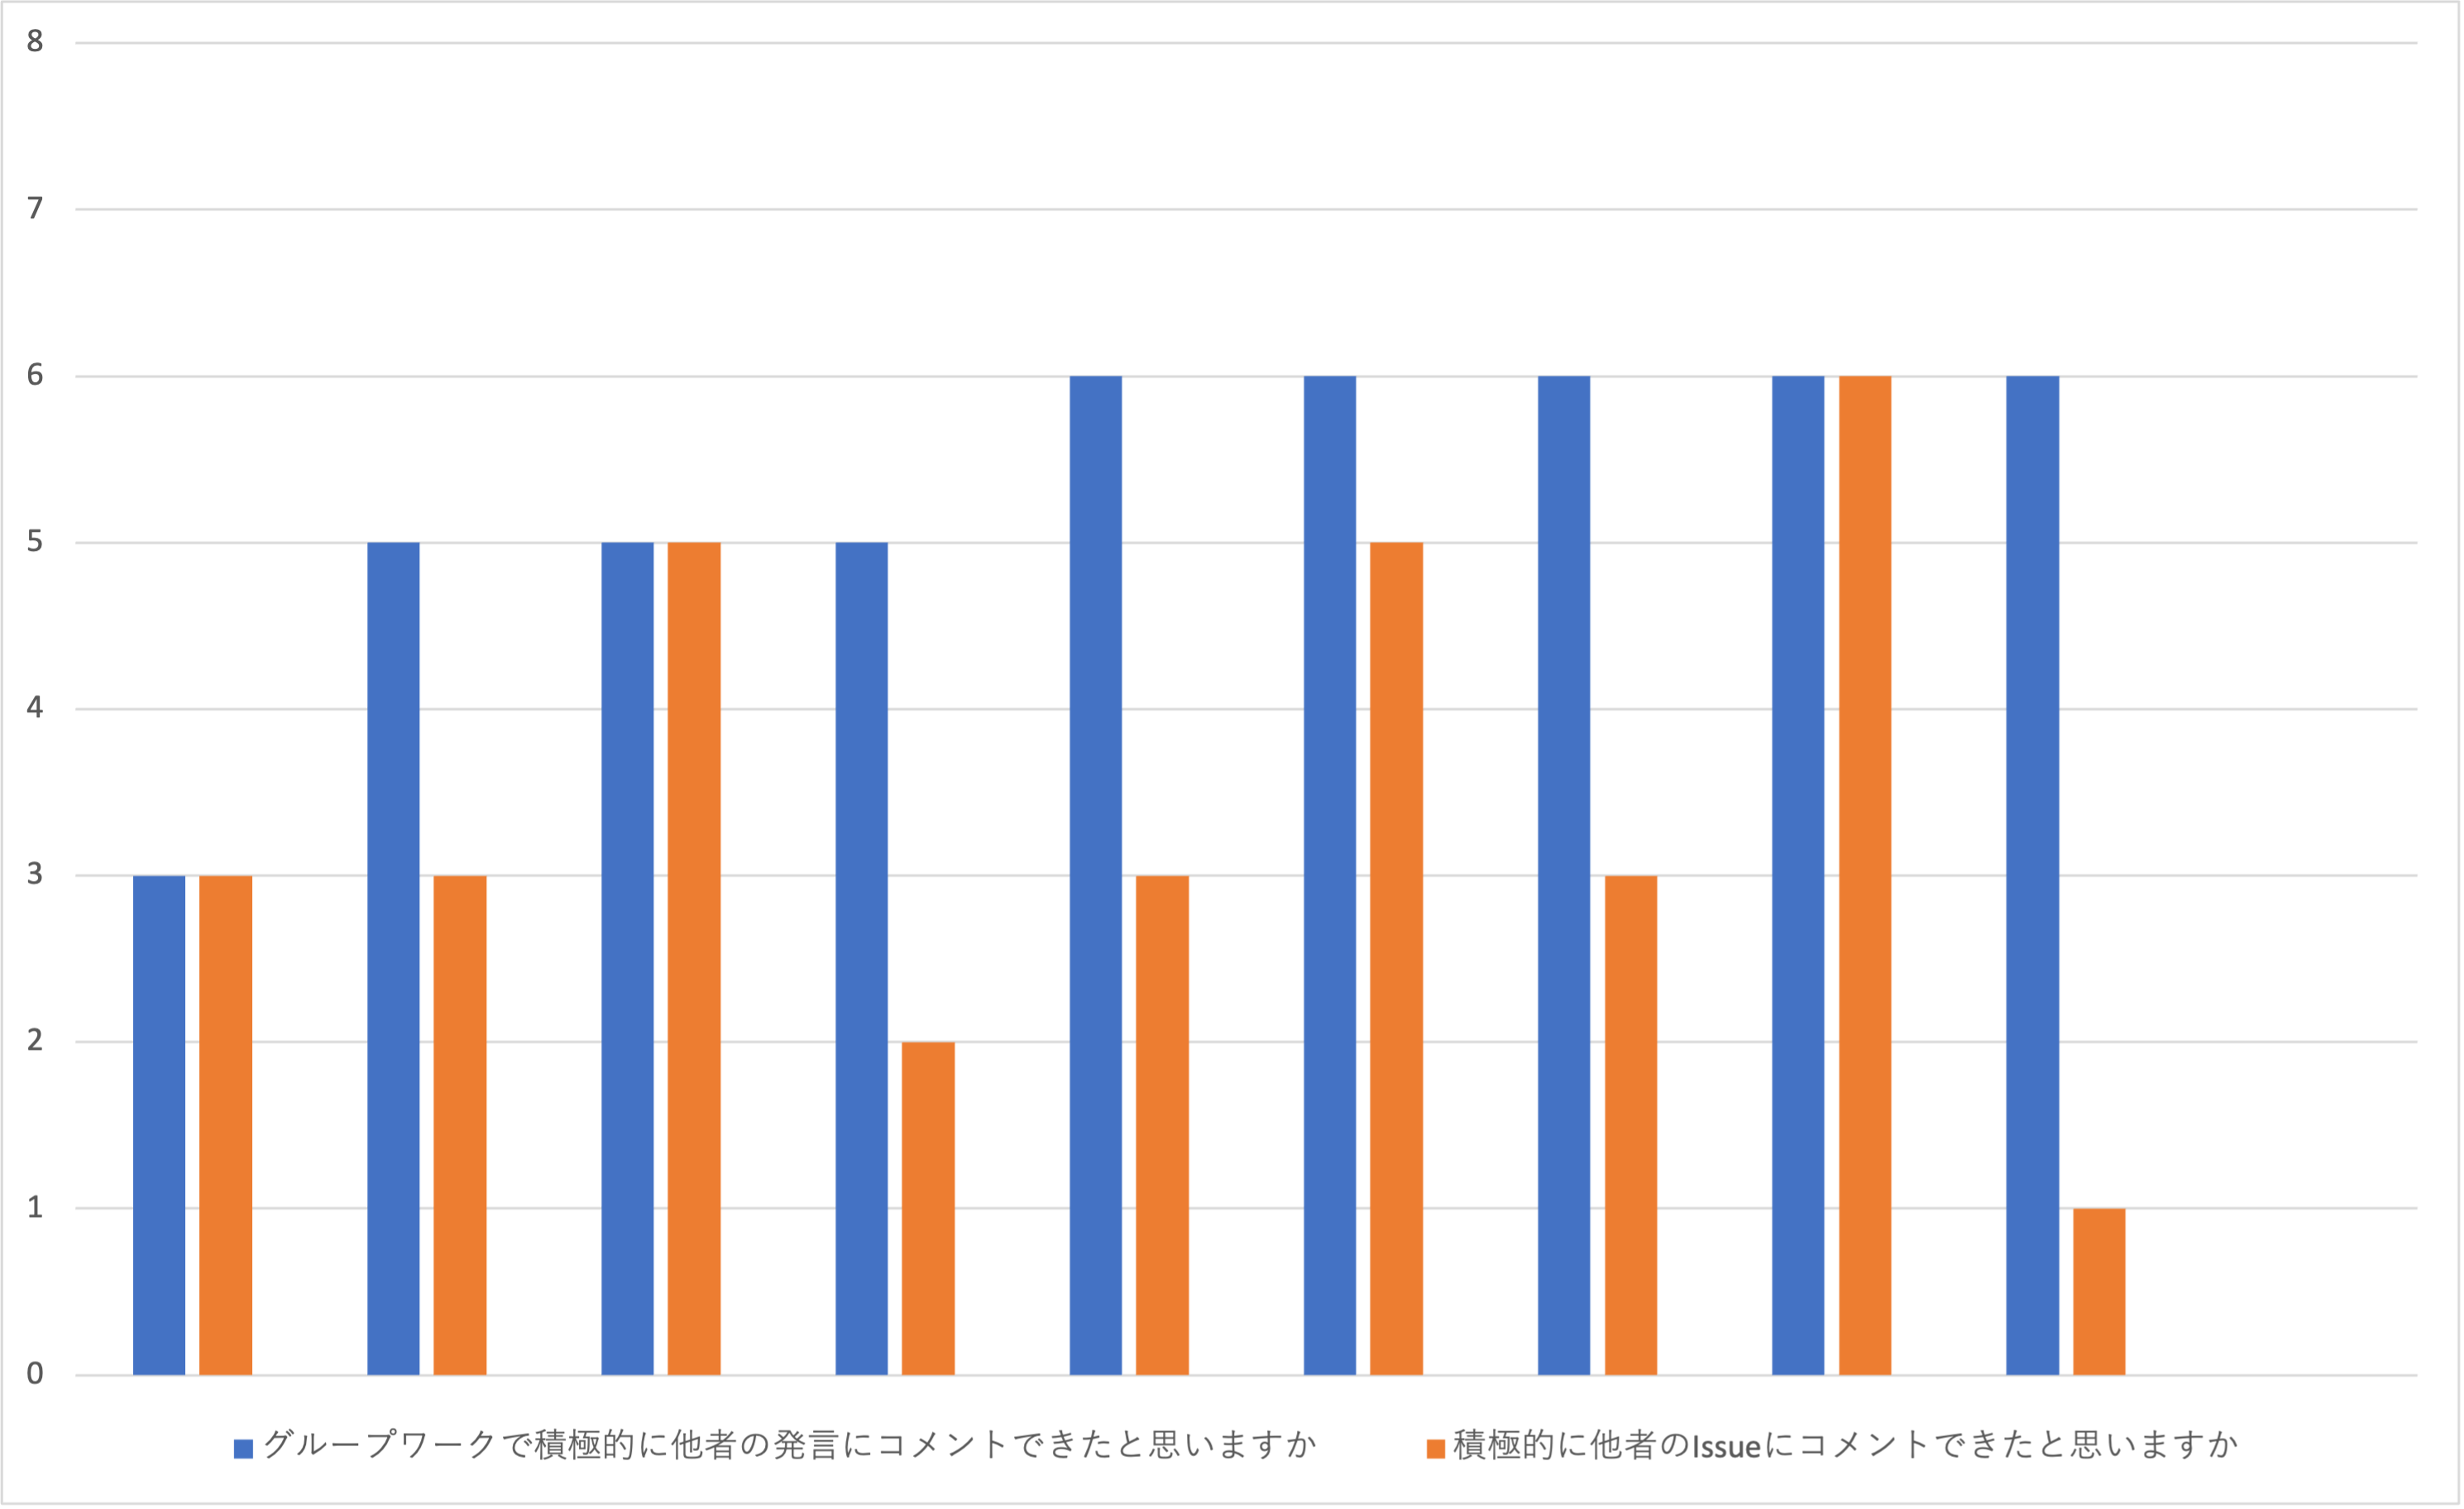
\includegraphics[width=1\linewidth]{img/gh_vs_gw_not.png}
    \caption{ワークシートが順調に進まなかった学生}
    \label{fig:gh_vs_gw_not}
  \end{minipage}
\end{figure}

多くの学生が,グループワークでは積極的に他者の発言にコメントできたと感じているが,本検証でのGitHub Issuesで他者にコメントできなかったと感じている.「ワークシートが順調に進んだ学生」の方が「ワークシートが順調に進まなかった学生」に対して,GitHub Issuesで積極的に他者の問題にコメントできていなかったと感じていることが分かる.

\section{興味,関心の多さと取り組みの多さの関係}

主体的な活動についての質問は,全て課外活動に相当するもの,かつプログラミングや技術に関する勉強会,個人学習に関する取り組みに関して質問した.これらの内容に,多くのチェックを行った学生を,「取り組みが多い学生」経験が多い学生と表記する.興味,関心について測定するために, プログラミングや技術に関する勉強会,個人学習に関する興味,関心に関する質問をした.これらの内容に,多くの回答項目にチェックを行った学生を,「興味が多い学生」と表記する.興味関心に関する設問の回答項目は22項目である.主体的な活動に関する回答項目は13項目である.

以下の図\ref{fig:kyoumi_vs_torikumi_yes}のグラフに「ワークシートが順調に進んだ学生」の課外活動の取り組みに関する設問と課外活動に関する興味,関心についての設問の関係をグラフで示す.図\ref{fig:kyoumi_vs_torikumi_not}のグラフに「ワークシートが順調に進まなかった学生」の課外活動の取り組みに関する設問と課外活動に関する興味,関心についての設問の関係をグラフで示す.それぞれのグラフの縦軸は,学生の課外活動に関する興味,関心の個数,課外活動の取り組みの個数を示し,横軸は学生ごとの回答を示している.

\begin{figure}[htbp]
  \begin{minipage}[c]{.5\linewidth}
    \centering
    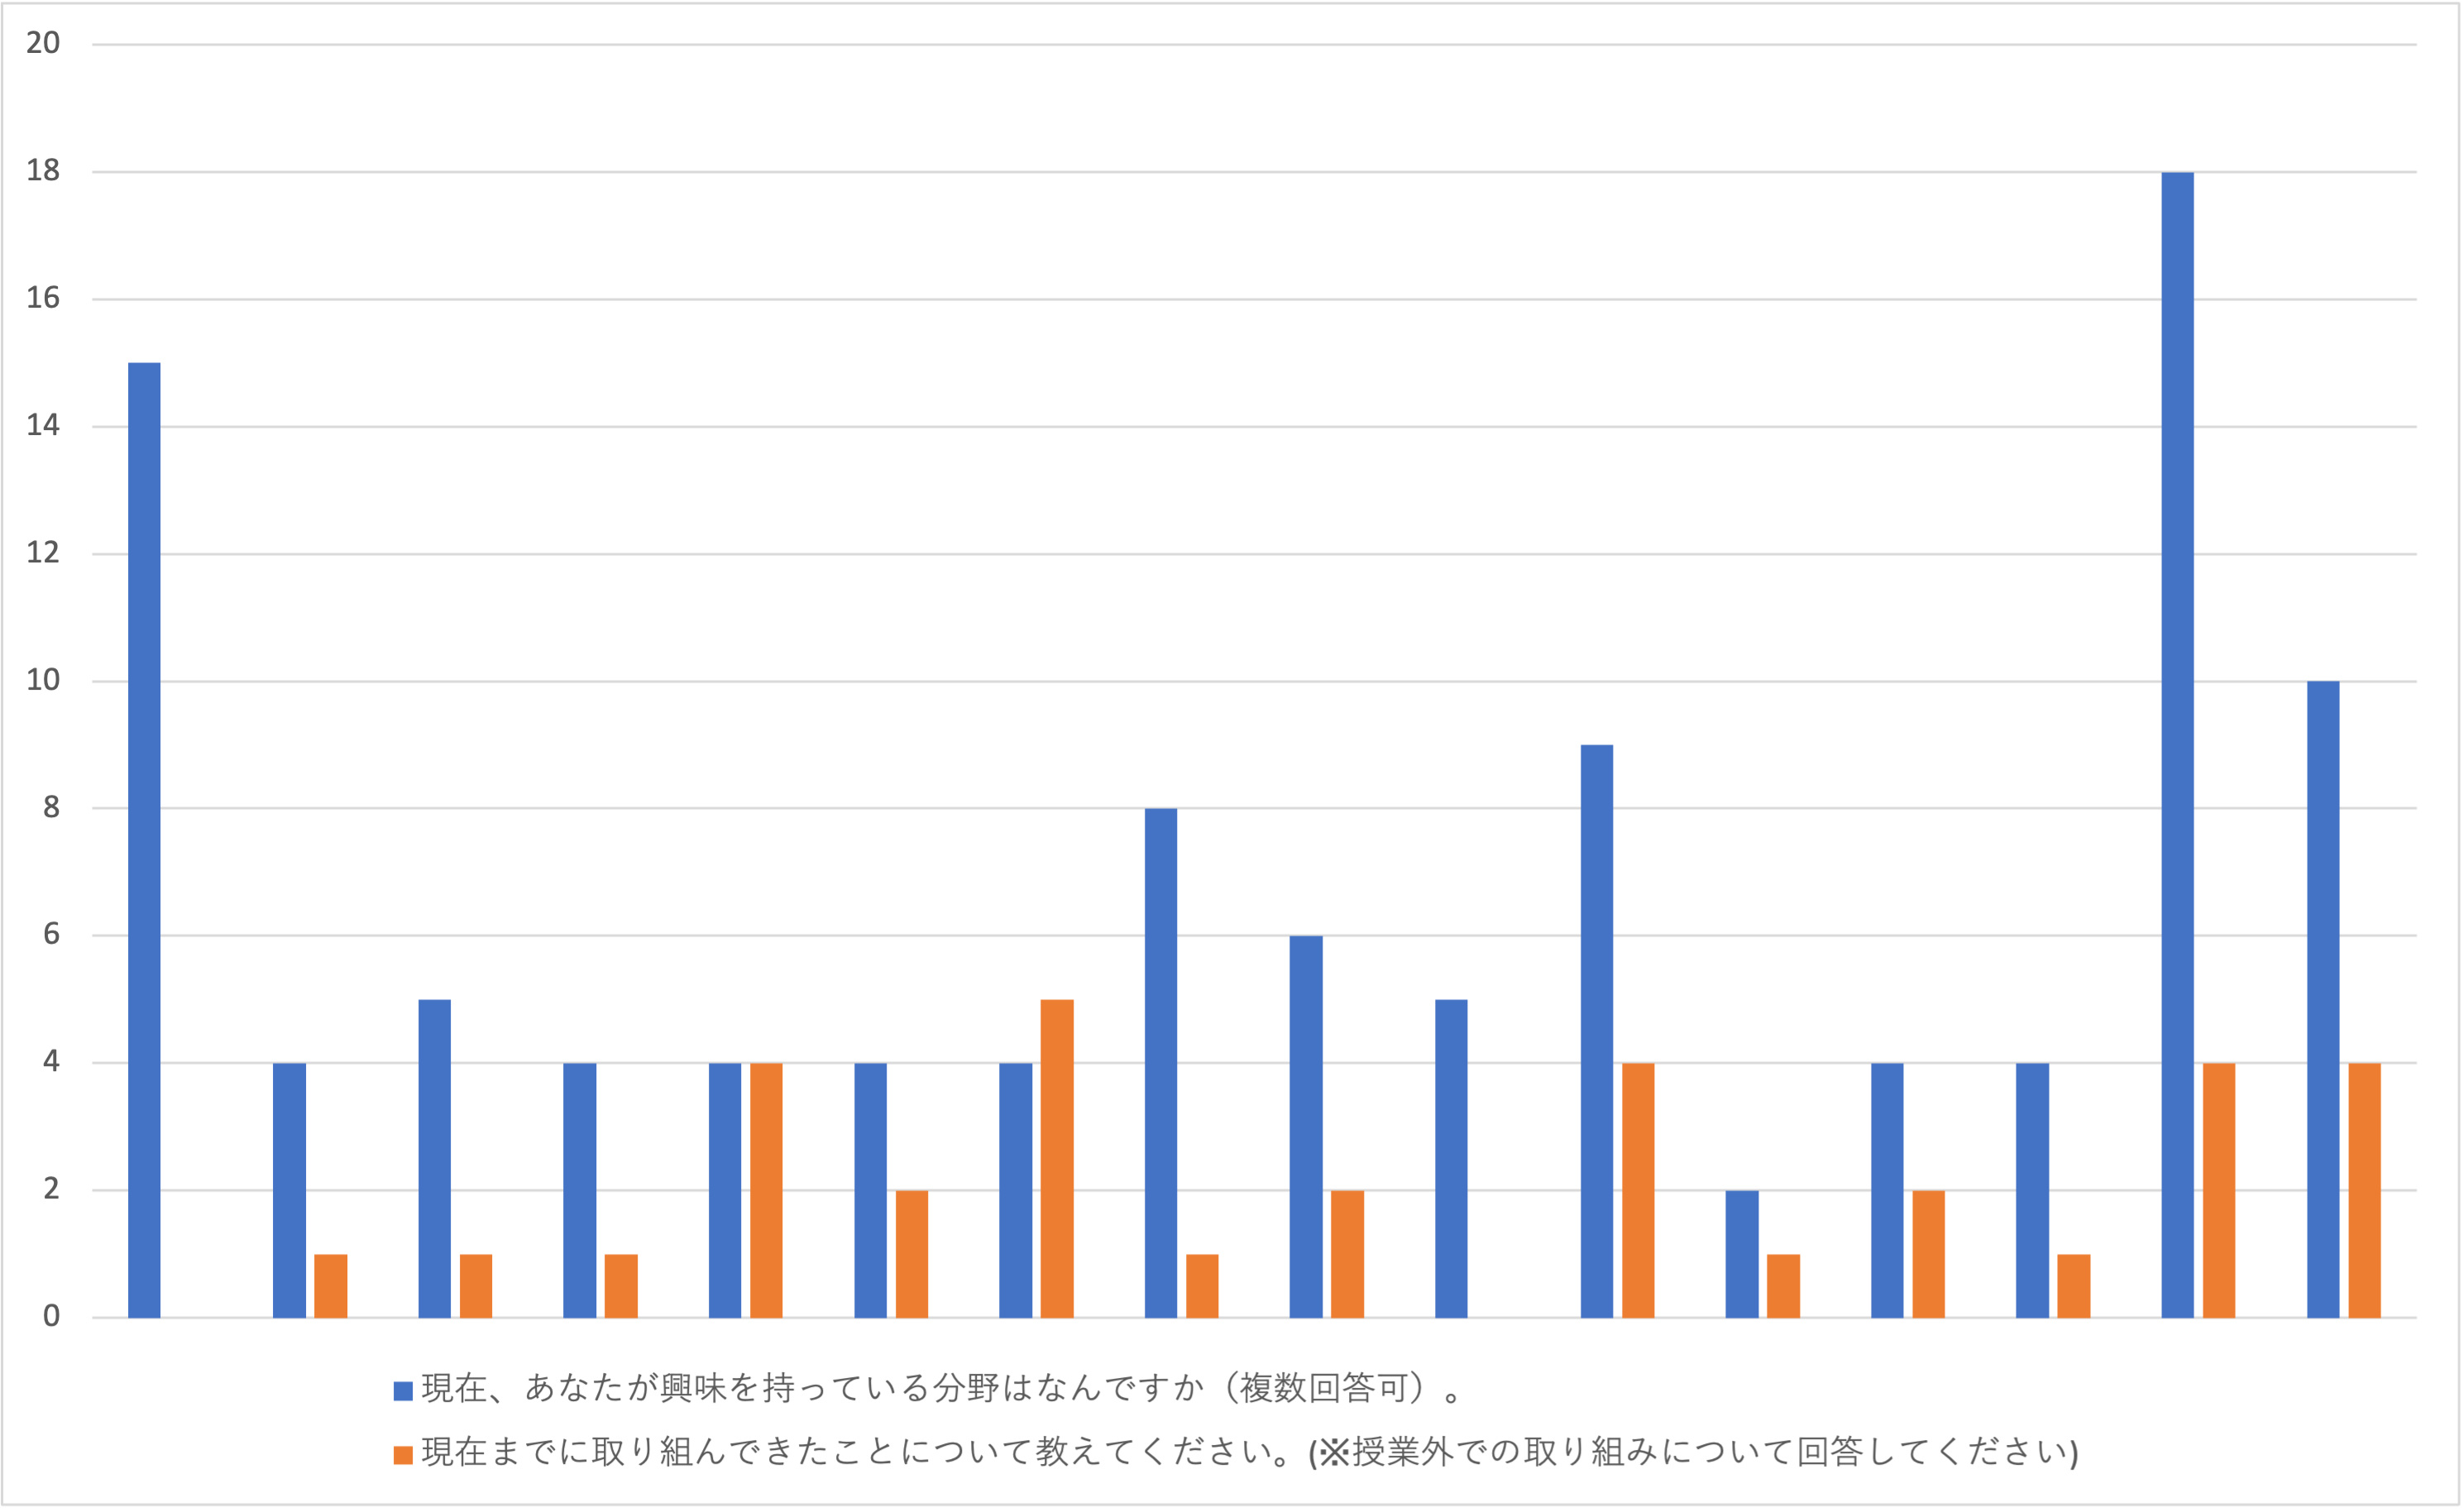
\includegraphics[width=1\linewidth]{img/kyoumi_vs_torikumi_yes.png}
    \caption{ワークシートが順調に進んだ学生}
    \label{fig:kyoumi_vs_torikumi_yes}
  \end{minipage}
  \begin{minipage}[c]{.5\linewidth}
    \centering
    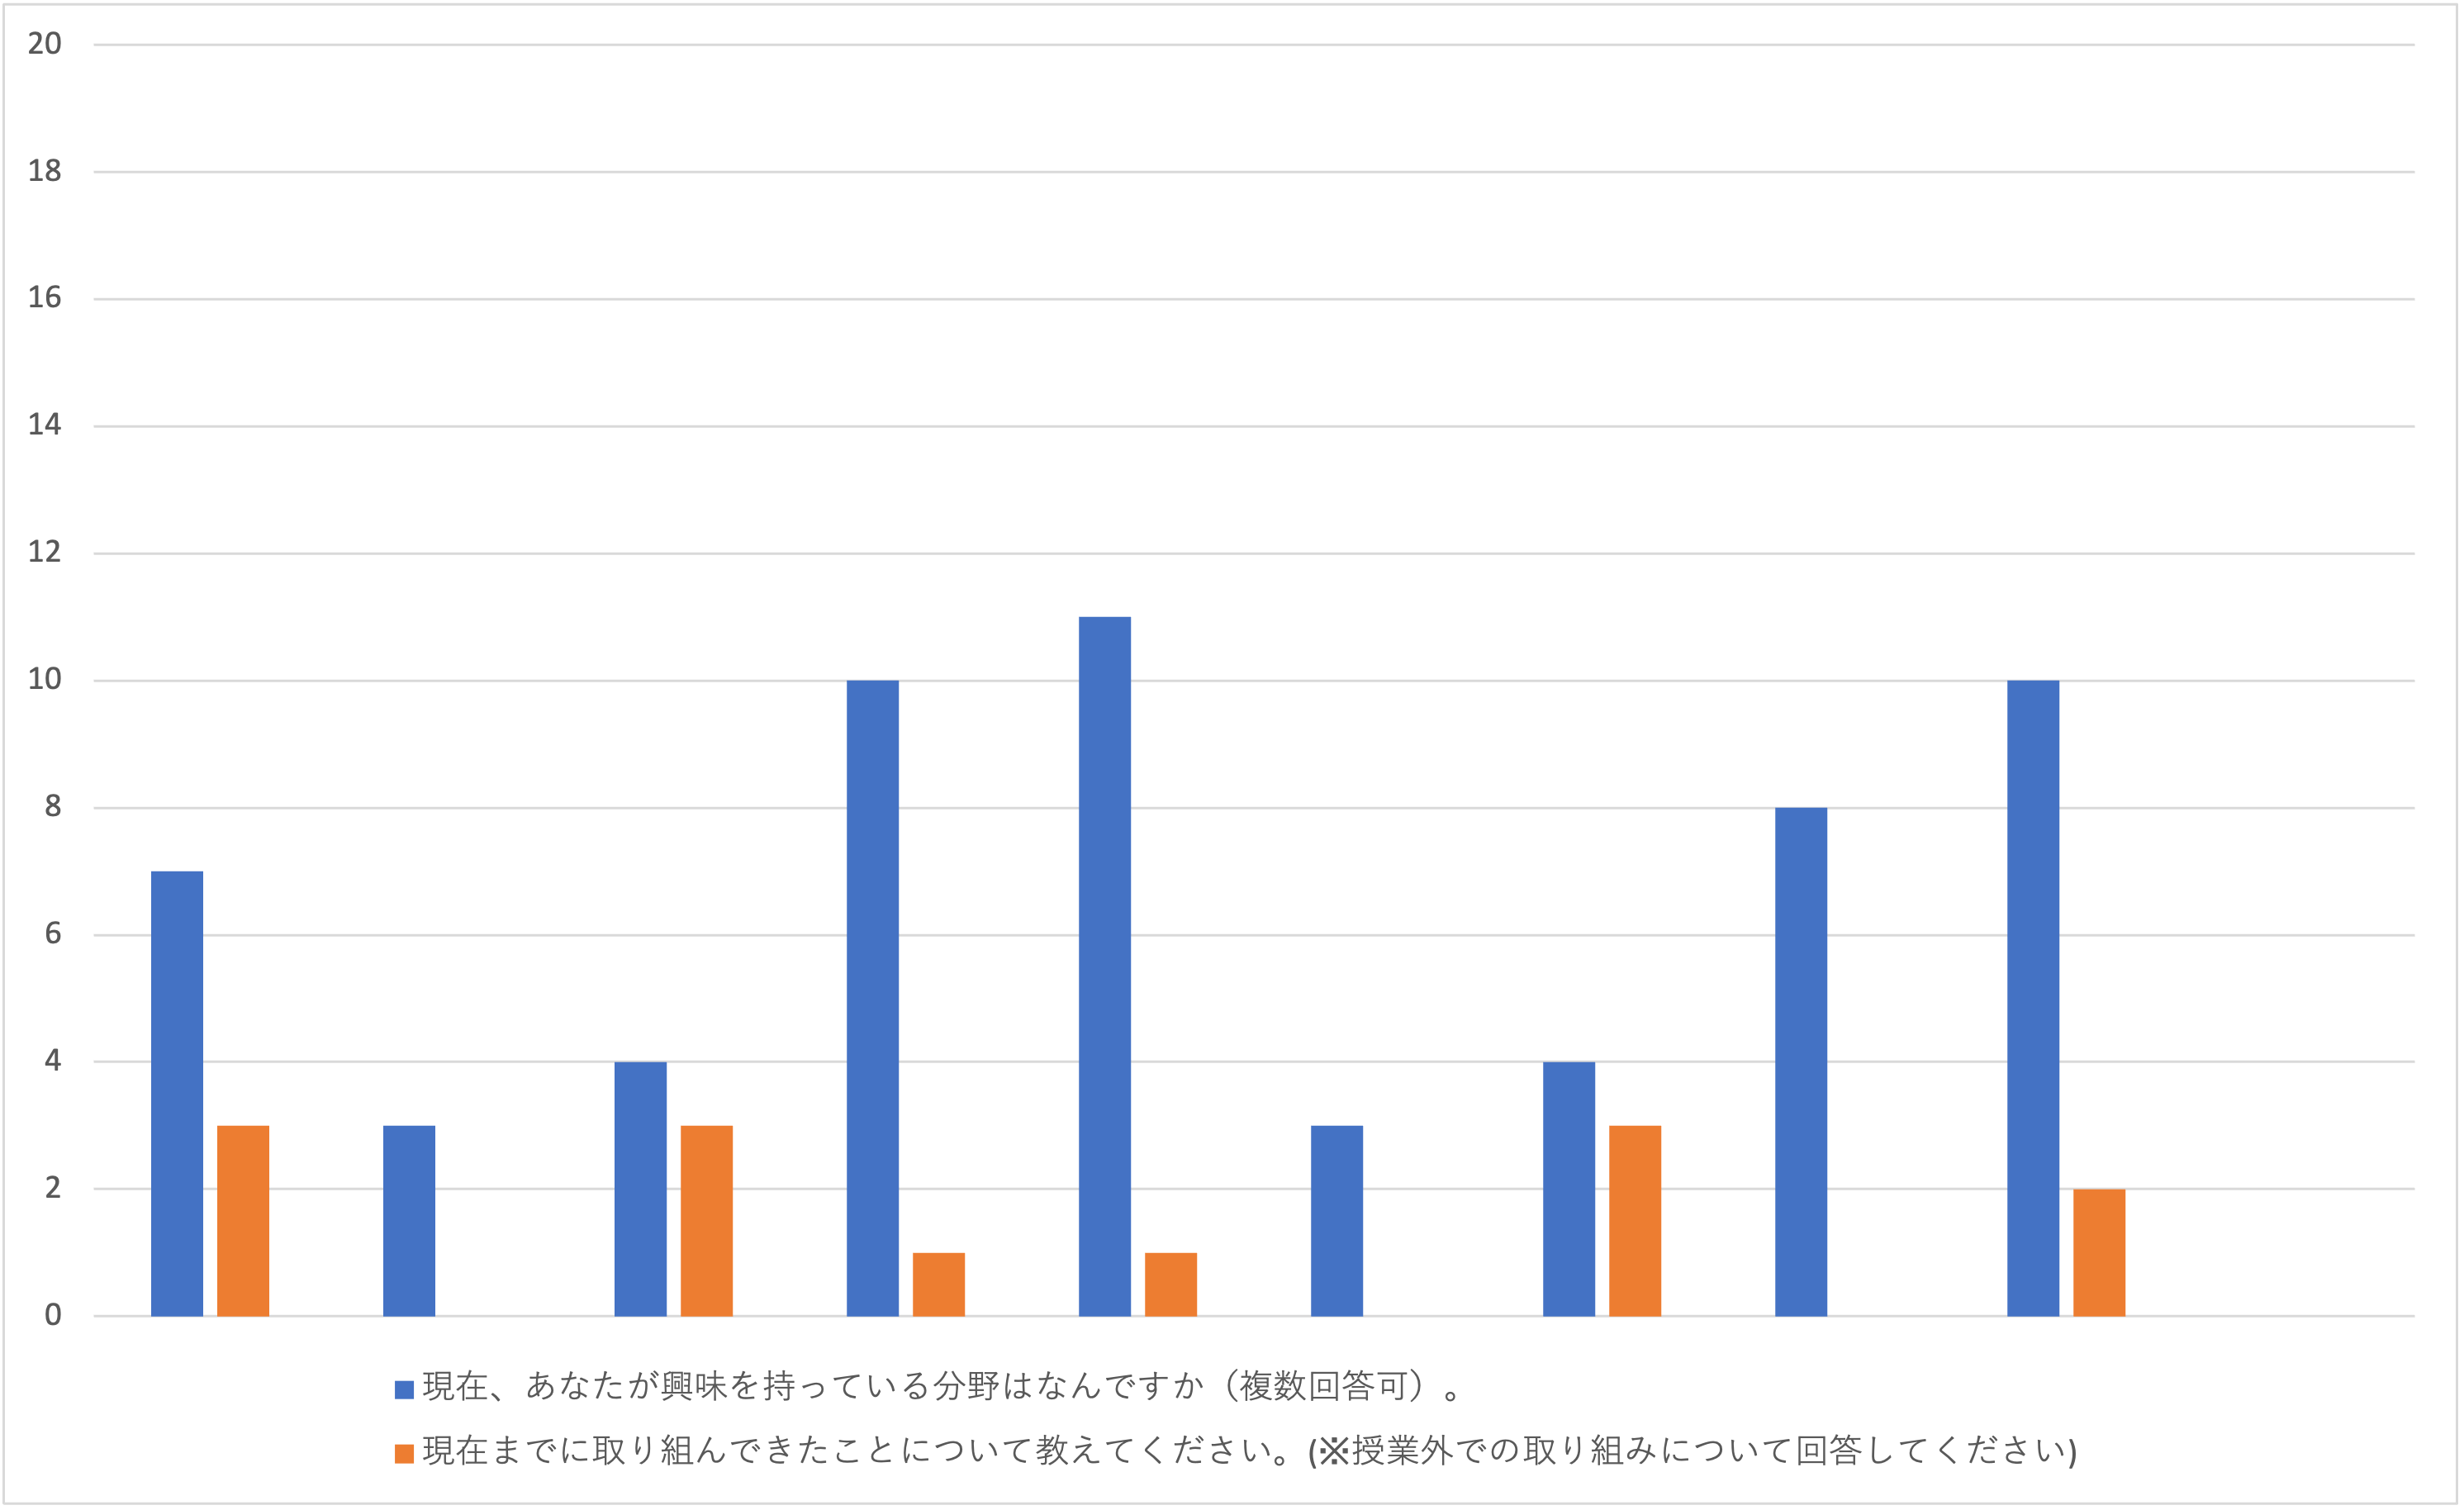
\includegraphics[width=1\linewidth]{img/kyoumi_vs_torikumi_not.png}
    \caption{ワークシートが順調に進まなかった学生}
    \label{fig:kyoumi_vs_torikumi_not}
  \end{minipage}
\end{figure}


「ワークシートが順調に進んだ学生」と「ワークシートが順調に進まなかった学生」のどちらも,興味,関心の多さと取り組みの多さの関係はなかった.どちらの学生も,課外活動の取り組みの個数の方が課外活動に関する興味,関心の個数より少ない傾向がある.

\newpage

\section{チェックツールの利用についての結果}

「テストツール(コマンドラインのチェッカー)は役に立ったと思いますか」の設問に対しての回答を「ワークシートが順調に進んだ学生」と「ワークシートが順調に進まなかった学生」に分けて示した.表\ref{tab:grech_yes}の左の表が「ワークシートが順調に進んだ学生」の結果を示しており,表\ref{tab:grech_no}の右の表では「ワークシートが順調に進まなかった学生」の結果を示している.

\begin{table}[htbp]
  \begin{minipage}[c]{0.5\hsize}
        \caption{ワークシートが順調に進んだ学生}
        \label{tab:grech_yes}
        \centering
        \begin{tabular}{|c|c|c|} \hline
        項目 & 人数 & 割合\\ \hline
        とても思う & 2人 & 12.5\% \\ \hline
        思う & 1人 & 6.3\% \\ \hline
        すこし思う & 3人 & 18.8\% \\ \hline
        あまり思わない & 2人 & 12.5\% \\ \hline
        思わない & 0人 & 0\% \\ \hline
        全く思わない & 0人 & 0\% \\ \hline
        使っていない & 8人 & 50\% \\ \hline
        \end{tabular}
    \end{minipage}
    \begin{minipage}[c]{0.5\hsize}
        \caption{ワークシートが順調に進まなかった学生}
        \label{tab:grech_no}
        \centering
        \begin{tabular}{|c|c|c|} \hline
        項目 & 人数 & 割合\\ \hline
        とても思う & 0人 & 0\% \\ \hline
        思う & 4人 & 44.4\% \\ \hline
        すこし思う & 2人 & 22.2\% \\ \hline
        あまり思わない & 0人 & 0\% \\ \hline
        思わない & 1人 & 11.1\% \\ \hline
        全く思わない & 0人 & 0\% \\ \hline
        使っていない & 2人 & 22.2\% \\ \hline
    \end{tabular}
  \end{minipage}
\end{table}


「ワークシートが順調に進んだ学生」の3割以上の学生が役に立ったと思っている.一方で,「ワークシートが順調に進まなかった学生」は6割以上の学生が役に立ったと思っている. 

「ワークシートが順調に進んだ学生」の結果では,半数の学生が利用していないと回答している.「ワークシートが順調に進まなかった学生」の結果では,2割の学生が利用していないと回答している.

\section{技術ブログの執筆ついての結果}\label{kekka_blog}

本検証内で学生に対し,技術ブログを書くことを促した.その結果,3名(12\%)の学生が技術ブログを執筆した.

執筆した学生の一人にインタビューで執筆に至った経緯について調査した.執筆した学生は,教員からの助言により,自信がついたため執筆した.また,執筆する内容についても具体的な助言があったため執筆したと回答した.

\section{自由記述}

前半の演習終了後に行ったアンケートの自由記述の回答について述べる.「非同期なコミュニケーションと同期的なコミュニケーション」と「演習に関する感想」についての結果を以下で示す.

\subsection{非同期なコミュニケーションと同期的なコミュニケーション}

「オペレーティングシステムの演習でのテキストコミュニケーションと比較し、会話でのコミュニケーションについての意見を教えてください。よかった点や難しかった点を教えてください。」の設問では以下の回答が得られた.

\begin{itemize}
\item 文字に起こすことで明確に言語化できる点ではテキストコミュニケーションの方が良いと思う。
\item テキストコミュニケーションと比較して会話だと話す内容を整理する時間がないので難しく感じる。特に話している途中で詰まって他者を待たせてしまう気まずさは苦手。良い点はリアルタイムで情報を更新しやすく訂正も楽な点。
\item 会話でのコミュニケーションでは直接話しながら問題の解決に取り組めるため、テキストと比べて素早く疑問を解消することができた。また相手の理解度に合わせて教える側が言い回しを変えることができることも利点である。一方疑問解消のやり取りがその場限りになってしまうため、テキストコミュニケーションのように長期的な疑問解決を図ることは難しいと感じた。
\item グループで一丸となって取り組む課題では会話でのコミュニケーションが必要だが、課題をそれぞれ黙々と取り組む課題ではテキストコミュニケーションで十分であると感じた。
\end{itemize}

個人で事象を整理してから質問できるため,他者の時間を奪うことなく進めることができるという意見があった.一方で,調べたことや問題を整理し,文章にすることが難しいという意見もあった.グループワークでは,話ながら状況を会話する相手と整理できることができるという意見もあった.

グループワークのような遅延なくコミュニケーションできる方が学生にとって簡単であるということがわかった.演習を個人で調査しながら行うことができる学生は,テキストコミュニケーションで十分であると感じている.

\subsection{演習に関する感想}

「オペレーティングシステムの演習についての感想を教えてください。」の設問では以下の回答が得られた.

\subsubsection{「ワークシートが順調に進んだ学生」の感想}

\begin{itemize}
\item ワークシートの誘導が丁寧で、わかりやすくシステム構築まで行けたので自信がついた。
\item 今までにないスタイルで課題に取り組めたので、楽しく知識をつけられたと思います
\item 普段自分が使用したり意識しないことを今回の演習で学べて、今後の開発で役に立つと考えた。また、コマンドを用いての操作に対して苦手意識を持っていたが、演習前よりも苦手意識がなくなったと感じた。
\item 資料の見落としを少なくすることが重要だが、調べることも重要だと感じた。環境を見比べることや、解決策が自分に合っていないことも多く難しさも感じた。
\item コマンド操作への苦手意識がなくなったため良かった。ワークシートが、使用するコマンドなどを一つずつ理解しながら進められるように作られていたため、完成したときに達成感があった。
\end{itemize}

\subsubsection{「ワークシートが順調に進まなかった学生」の感想}

\begin{itemize}
\item LAMP環境の構築を自分のペースで作成できたためとても良い経験になったが、分からない部分は自力で答えにたどりつけない分野であると感じたので、書籍や先輩、教授から知識を身につける必要があると感じた。
\item 一つのエラーの対応のために授業の時間を丸々投げてしまったこともありましたが、何とか完成できた時の達成感はとても良かったです。
\end{itemize}

「ワークシートが順調に進んだ学生」は,資料の全てに目を通した上で問題点の調査を行っていることがわかる.また,資料の各項目の仕組みなどについて演習を行いながら理解できたことに対して達成感を感じている.

一方で,「ワークシートが順調に進まなかった学生」は,スチューデントアシスタントや教員の助力を得て,演習を完了できたことに達成感を感じている.また,「書籍や先輩、教授から知識を身につける必要」と述べており,自身の学習ではなく,直接的な他者の助力により,知識習得を行いたいと思っている.

\section{GitHub Issuesの結果}

18件の投稿があった.適切に「発生している事象」「調べたこと」「考えられる原因」が記載されたコメントもあったが,エラーログのみが記載されたコメントもあった.

図\ref{fig:lognomi}に示したGitHub Issuesでは,現在の状況ややりたいことを説明する内容は記載されていたが,なぜ起きているのかの考察やどのような操作を行ったのかの説明がなかった.また,作成したテンプレートを無視したGitHub Issuesであることが分かる.実行ログや現在の状況をスクリーンショットのみで他者に問題解決を求めている.

\begin{figure}[H]
\begin{center}
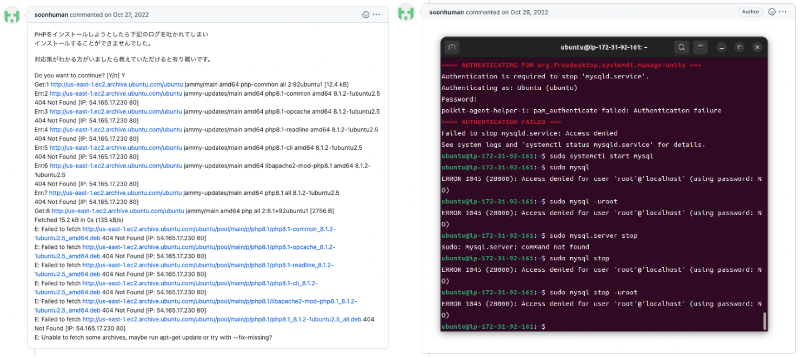
\includegraphics[width=140mm]{./img/lognomi.png}
\caption{情報が少ないコメント}
\label{fig:lognomi}
\end{center}
\end{figure}

学生同士でコミュニケーションが行われた様子を図\ref{fig:issuehennsin}に示す.

\begin{figure}[H]
\begin{center}
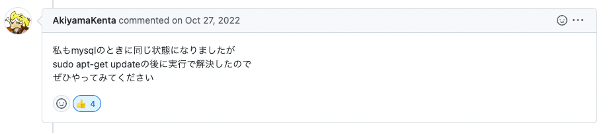
\includegraphics[width=140mm]{./img/issuehennsin.png}
\caption{GitHub Issuesでのコミュニケーションの様子}
\label{fig:issuehennsin}
\end{center}
\end{figure}

学生からのコメントに対してスチューデントアシスタントや教員がコメントすることもあった.教員やスチューデントアシスタントのコメントで学生が問題を解決できたこともあった.一方で,学生同士でのコミュニケーションにより学生が問題を解決できたこともあった.図\ref{fig:grechissue}では,本検証環境で導入した演習環境チェックツールの実行結果を元に原因を考察し,自己解決した様子を示す.

\begin{figure}[H]
\begin{center}
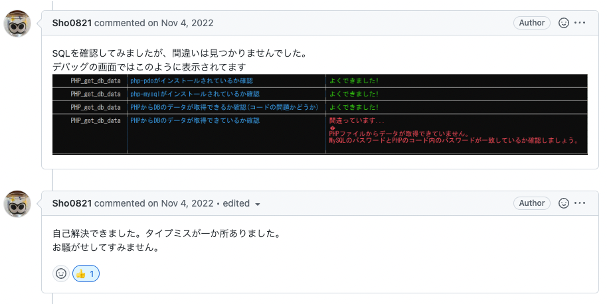
\includegraphics[width=140mm]{./img/grechissue.png}
\caption{自己解決されたコメント}
\label{fig:grechissue}
\end{center}
\end{figure}


\section{インタビューの結果}

自由課題に取り組む期間内に4人にインタビューを行った.インタビューの対象者は,GitHubのコメント履歴や技術ブログの執筆の有無,アンケートの結果から,傾向が異なる学生を選択した.インタビュー調査は1対1の対面方式で行い,その内容は音声で記録した.それぞれの学生はアンケートより異なる特性がある.ポジティブな内容とネガティブな内容についてそれぞれ示す.

「演習に関する自信について」「最終課題について」「達成感,楽しさ,満足感について」「今まで取り組んできたこと」「これから取り組みたいこと」についての結果を以下に示す.

\subsection{演習に関する自信について}

\begin{itemize}
\item 「LAMP環境の構築を行ったことで,データベースについて理解が深まり,PHPで実装したデータベースとの連携をPythonを用いて最終課題でも応用でもできそうだと感じた.」
\item 「LAMP環境の構築がうまくいかず,エラーで詰まった.とても苦痛だった.」
\end{itemize}

\subsection{最終課題について}\label{saisyuunituite}

\begin{itemize}
\item 「LAMP環境の構築では行っていない新しい内容に挑戦している.最終課題で取り組んでいる内容を技術ブログで執筆した.」
\item 「最終課題についても詳しく教えて欲しい.自分で学んだ技術を応用しながら課題に取り組むことは難しい.」
\end{itemize}

\subsection{達成感,楽しさ,満足感について}

\begin{itemize}
\item 「基礎を自身で理解を深めながら学び,知識を身につけていく過程で興味を持っていく.」
\item 「簡単な問題を時間を掛けずに多く解決させた方が達成感を感じる.」
\end{itemize}

\subsection{今まで取り組んできたこと}

\begin{itemize}
\item 「学内のチームでの活動で,多くの人から期待されてシステム開発を行えた.期待されたことで,自身で学びながら活動に貢献できた.」
\item 「大学内外の課外活動に参加したことがない.」
\end{itemize}

\subsection{これから取り組みたいこと}

\begin{itemize}
\item 「友人と参加できる活動であれば大学内外問わず参加したい.先生などからの紹介があれば一人でも学外の活動に参加したい.」
\item 「授業外でプログラミングをしたいと思っているが,なかなか取り組めない.プログラミングを行うサークルや学内の課外のシステム開発の活動に参加することは抵抗がある.授業時間外に拘束されることが不満である.」
\end{itemize}

知識習得に意欲的な学生と,そうでない学生がいることが分かった.知識習得に意欲的な学生は,能動的に課外活動で自身の成長に時間を使っている.一方で,課外活動に興味を示さない学生や授業外で時間を使うことに抵抗がある学生もいる.

知識習得に意欲的な学生は,知識習得にかかる時間に対して許容している.一方で,知識習得に時間がかかることや,達成感を得られるまでに時間がかかることに不満を感じる学生もいる.周囲から期待されることや教員などからの助言があることが課外活動に取り組むきっかけであることが分かった.

\section{演習授業後半の成果物の結果}

後半の演習では,学生自身で課題を設定し,自由にアプリケーションの構築を行うようにした.その成果物についての結果を述べる.

\begin{itemize}
\item PHPを書いたことがない学生が,LAMP構成のアプリケーション構築演習でPHPを知ったことでPHPで課題に取り組んだ学生がいた.
\item 前半のLAMP構成のアプリケーション構築演習や教員が提示したアプリケーション以外の課題を設定し取り組んでいる学生がいた.
\item 本検証で学習していないAWSのサービスやAWS以外のサービスを用いて開発を行った学生がいた.
\item 作成したアプリケーションについての説明資料とアプリケーションのソースコードをGitHubで公開した学生がいた.
\item \ref{kekka_blog}で述べた本検証内で執筆した学生の技術ブログを参考に課題に取り組んでいる学生がいた.
\item 教員が提示した資料を参考にアプリケーションの構築に取り組んだ学生がいた.
\item アプリケーションを満足に完成させることができなかった学生もいた.
\end{itemize}

\section{前年度のアンケートと比較した結果}

前年度の今年度の本授業に対して学生が期待したことについて学ぶことができたかについての匿名アンケート結果を示す.このアンケートは,第15回目の授業終了後に行った.「授業をつうじて伸ばしたいと思ったスキルが伸びましたか」の設問に対しての学生の回答を以下の表\ref{tab:zennnenn_konnnenndo_hikaku}に示す.前年度のアンケート回答者数は22人,今年度は19人が回答した.

\begin{table}[htbp]
  \begin{minipage}[c]{0.5\hsize}
        \caption{前年度}
        \label{tab:zennnenn_konnnenndo_hikaku}
        \centering
        \begin{tabular}{|c|c|c|} \hline
        項目 & 人数 & 割合\\ \hline
        とても伸ばせた & 3人 & 13.6\% \\ \hline
        伸ばせた & 16人 & 72.7\% \\ \hline
        伸ばせなかった & 3人 & 13.6\% \\ \hline
        全く伸ばせなかった & 0人 & 0\% \\ \hline
        \end{tabular}
    \end{minipage}
    \begin{minipage}[c]{0.5\hsize}
        \caption{今年度}
        \label{tab:zennnenn_konnnenndo_hikaku}
        \centering
        \begin{tabular}{|c|c|c|} \hline
        項目 & 人数 & 割合\\ \hline
        とても伸ばせた & 9人 & 47.4\% \\ \hline
        伸ばせた & 9人 & 47.4\% \\ \hline
        伸ばせなかった & 1人 & 5.3\% \\ \hline
        全く伸ばせなかった & 0人 & 0\% \\ \hline
        \end{tabular}
  \end{minipage}
\end{table}

「伸ばしたいと思った(思っていた)スキルについて教えてください」の設問では,前年度と今年度の学生のどちらも「システムがネットワークに繋がる仕組み」「クラウド構築のスキル」「複数のシステム・サービスを連携して一つのシステムを作るスキルや、サーバの構築スキル」などの回答していた.本検証を行った講義に学生が求める授業内容は前年度と今年度で大きな差がないと考えられる.

前年度と比較し,今年度の学生は授業冒頭で思っていた学びたいことを本演習授業を通じて伸ばせたと感じている学生が増加した.

\chapter{結論}

\section{考察}

ここでは,\ref{hyouka}で示した結果を元に考察を述べる.

\subsection{達成感や自信について}

本研究で提案する学習モデルをサーバ構築演習に適用した.その結果,学生のARCSモデルの関連性,注意,自信の項目を向上させることができた.これは,インタビューやアンケートの結果から,他のプログラミングの授業との関連性が明らかになったことや,周辺知識が身についたことが要因だと考えられる.また,ワークシートで提示された課題が完了できたことが自信につながっていることも考えられる.

前年度の演習授業と比較し,今年度の演習ではLAMP構成のアプリケーション構築演習とオープンソースソフトウェア開発プロセスの要素を授業に取り入れた.LAMP構成のアプリケーション構築演習を行い基礎の学習を行ったことで,学生が授業冒頭で求めていたスキル習得が行えたと考えられる.学生が自身で課題を設定し,自主的に取り組む課題の前に基礎的な学習を演習授業で学ぶことは,学生が成長を実感することにつながると推測される.

\subsection{学習プロセスについて}

一部の学生は,学生自身で学びの経路を確認することはできていなかったと推測される.整理した情報や知識を文章にしてGitHub Issuesのコメントに書き込むことができていなかった.また,知識や考察,情報の妥当性の評価を行うことが難しいと感じており,テキストコミュニケーションでは,学生が伝えたい情報が十分に伝わらないことがわかった.情報を整理しテキストで表現できない学生は,学習プロセスを自身で理解できていないと考えられる.または,知識や習得した情報を適切にまとめる能力が低いと考えられる.

\subsection{非同期なコミュニケーションと同期的なコミュニケーションの特性}

アンケートやインタビューで分かった非同期なコミュニケーションと同期的なコミュニケーションの特性を表\ref{tab:hidouki_douki}に示した.それぞれのコミュニケーションの「学生の他者貢献に対する積極性」,「学生が感じるコミュニケーションの難易度」,「コミュニケーションを行い問題解決するまでの時間」,「学生が発言することに対して抵抗があるか」のについて示した.

\begin{table}[H]
\caption{非同期なコミュニケーションと同期的なコミュニケーションの特性}
\label{tab:hidouki_douki}
\centering
\begin{tabular}{|c|c|c|c|c|} \hline
\begin{tabular}{c}\end{tabular} & \begin{tabular}{c}積極性\end{tabular} & \begin{tabular}{c}難易度\end{tabular} & \begin{tabular}{c}時間\end{tabular} & \begin{tabular}{c}抵抗の有無\end{tabular}\\ \hline

\begin{tabular}{c}同期的な\\コミュニケーション\end{tabular} & \begin{tabular}{c}高い\end{tabular} & \begin{tabular}{c}低い\end{tabular} & \begin{tabular}{c}短い\end{tabular} & \begin{tabular}{c}ない\end{tabular}\\ \hline
\begin{tabular}{c}非同期な\\コミュニケーション\end{tabular} & \begin{tabular}{c}低い\end{tabular} & \begin{tabular}{c}高い\end{tabular} & \begin{tabular}{c}長い\end{tabular} & \begin{tabular}{c}ない\end{tabular}\\ \hline
\end{tabular}
\end{table}

テキストコミュニケーションは情報共有はグループワークと比較し,積極的に情報共有が行われにくいことが分かった.また,GitHub Issuesのコメントには,自身の考察や知識の情報がなく,他者に情報が十分に伝達できないことがあった.一方で,テキストコミュニケーションの時間や場所に縛られないことや,情報を整理する時間が十分にあることなどをメリットに感じつつ,テキストコミュニケーションは同期的なコミュニケーションと比較し難しいと感じている学生が多い.アンケートの結果から,対話する相手の知識レベルや抱えている課題を認知するまでの時間が影響していると考えられる.

主体的に取り組まない学生は,問題解決までに時間がかかるにつれ不満に感じるようになる.そのため,テキストコミュニケーションより,グループワークのような同期的なオーラルコミュニケーションの方がコミュニケーションに時間がかからず,苦痛を感じにくい.また,\ref{gw_tc_diff}で述べたように課題に対して個人で取り組むことができる学生が積極的に発言する傾向があるグループワークのようなオーラルコミュニケーションの方がテキストコミュニケーションと比較し,苦痛を感じにくいと考えられる.

\subsection{認知プロセスの外化について}\label{end_ninnti_gaika}

講義内で,課外活動である技術ブログの執筆を勧めたことで,4名の学生が執筆に取り組んだ.執筆に取り組んだ学生は,アンケートの結果やインタビューの結果から,多くのことに興味がある学生や,興味があることは少ないが特定のことを深く学ぶことを好む学生が執筆していた.講義内で,執筆に対する心理的なハードルを下げたことが効果的に働き,学生が主体的に技術ブログを執筆することにつながった.

また,他の学生によって執筆されたブログを参考に最終課題に取り組んでいる学生がいた.この学生は,LAMP構成のアプリケーション構築後の時点で,後半の自由課題では教員から提案された課題に取り組もうとしていた.しかし,上記で述べたブログを参考に課題に取り組み,15回目の発表でブログを参考に作成したアプリケーションを発表していた.ブログではEC2上でチャットアプリのボット(Discord Bot)を動かすことについて情報がまとめられている.これは,能動的でない学生が,他の能動的な学生に影響されて取り組むようになった例である.

\subsection{課外活動に積極的な学生とそうでない学生の特性}

サーバ構築演習で課題を自身で設定し,取り組む学生は,課外活動で積極的に活動している傾向がある.また,教員が具体的な課外活動を示すことを積極的に行うことで,主体的に課外活動に取り組むようになると考えられる.一方で,サーバ構築演習で能動的に活動しない学生は,課外活動に対しても苦痛を感じていることが分かった.また,GitHub Issuesやインタビューから,基礎リテラシーが低く,認知プロセスの外化ができていない.派生知識に無関心であると考えられる.

課外活動に積極的に取り組み,それぞれの活動に時間をかける学生には,本研究で提案する学習モデルの効果があり,主体的な学習を促すことができた.本研究で提案する学習モデルでは,学生自身で問題を調査し,妥当性を評価することを学生に要求する.課外活動に積極的に取り組み,それぞれの活動に時間をかける学生は,本検証前から本研究で提案する学習モデルが要求する能力を身につけていたと考えられる.

\vskip\baselineskip

本研究では改善を図っていないが,学生によっては,大学の講義や演習で主体的に学ぶことを促される学習モデルに苦痛を感じる学生がいた.課外活動で主体的な活動を求められることには不満はない学生,課外活動でも主体的に学ぶことに不満を感じる学生がいた.「課外活動で主体的な活動を求められることには不満はない」学生は,興味がある分野であれば,十分なサポートが受けられる活動であれば,積極的に参加したい傾向がある.このような学生は,外部からの適切な働きかけにより,課外活動に取り組む傾向がある.一方で,「課外活動でも主体的に学ぶことに不満を感じる学生」は,外部からの働きかけに影響されて,講義外で活動したいと感じることが少ない.

また,本検証の自由課題でデータベースなどの連携を行うことができなかった学生や教員の十分な支援のもと完成させることができた学生がいた.このような学生は,他の授業のプログラミングの学習やデータベース,ネットワークなどの知識が身についておらず,他の授業の実践的な演習も理解しながら取り組めていないことが考えられる.本検証では,他の授業で学んだ知識や経験を前提に計画を行っていた.そのため,本演習で用いた資料で十分にプログラミングやデータベース,ネットワークについて解説しておらず,本検証の演習で苦戦したと考えられる.

\section{展望}

% 知識や情報を適切に表現できていない学生の文章を他者が理解し,適切な回答を行うことは困難であり,前述したように,問題解決までに時間が掛かり苦痛を与えることが分かった.改善として,テキストコミュニケーションで知識や情報を適切に表現できない学生に対して,個人で知識や情報を適切に表現する訓練を行う必要があると考えられる.改善として,前述の訓練の様子を図\ref{fig:tennbou2}に示す.提案として,このような学生には,他者に文章化し質問する前にGhat GPT\cite{bib:chatgpt}のような対話AIに文章で質問し,適切な回答が返ってくるまで文章を推敲しながら改善する支援システムを構築することで文章化する能力向上を図ることができると考えられる.

% \begin{figure}[H]
% \begin{center}
% 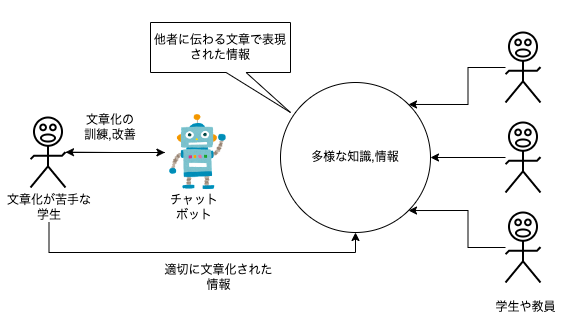
\includegraphics[width=120mm]{./img/tennbou2.png}
% \caption{情報の文章化の訓練}
% \label{fig:tennbou2}
% \end{center}
% \end{figure}

% \vskip\baselineskip

学生に課題を設定させて取り組ませる課題は,「主体的に課外活動に取り組まない傾向がある学生」や「自身で調査し理解を深めながら学習することに苦痛を感じる学生」にとっては難易度が高いことが分かった.また,教員が示す課題や知識習得に焦点を当てた課題に対して不満を感じる学生がいることが分かった.このような学生は,短時間で完成させることができる課題や自身が興味がある題材の課題に関心を示すと考えられる.このような学生にとって,\ref{end_ninnti_gaika}で述べた同じような感性を持つ学生が体系的に情報をまとめた資料に取り組むことが有効だと考える.提案として,図\ref{fig:tennbou1}のような学びの様子を示す.意欲的な学生らが好きな題材について体系的に情報をまとめ公開する.公開された情報を他の学生が参照し,短時間で再現し達成感を感じる.再現後に,理解を深め,自身で変更を加える.これにより,意欲的な学生から多様な情報やアイデアが提供され,意欲的でなかった学生も意欲的な学生に影響され課題に取り組むことができると考えられる.

\begin{figure}[H]
\begin{center}
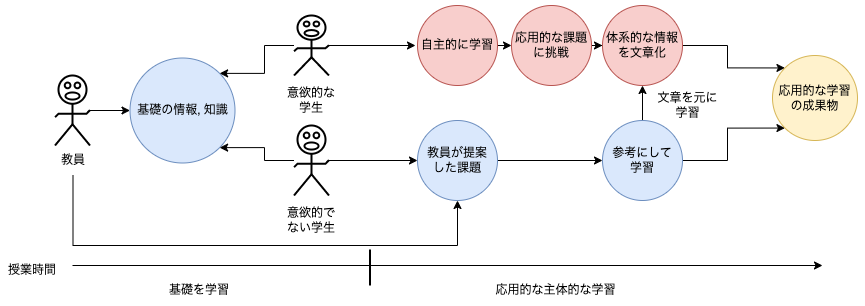
\includegraphics[width=140mm]{./img/tennbou1.png}
\caption{意欲的な学生と意欲的でない学生の学び}
\label{fig:tennbou1}
\end{center}
\end{figure}

%参考文献
\begin{thebibliography}{9}
\addcontentsline{toc}{chapter}{\bibname}

\bibitem{bib:oecd} 国立教育政策研究所(2013).「国立教育政策研究所プロジェクト研究 (平成21~25年度) 「教育課程の編成に関する基礎的研究」」.文部科学省.\\
\url{https://www.mext.go.jp/b_menu/shingi/chousa/shotou/095/shiryo/__icsFiles/afieldfile/2013/07/18/1336562_01_1.pdf},(参照 2023-02-06)

\bibitem{bib:mirai} 未来人材会議(2022).「未来人材ビジョン」.経済産業省.\\
\url{https://www.meti.go.jp/press/2022/05/20220531001/20220531001-1.pdf}

\bibitem{bib:kyouikutennkann} 文部科学省(2012).「新たな未来を築くための大学教育の質的転換に向けて~生涯学び続け、主体的に考える力を育成する大学へ~(答申)」.\\ \url{https://www.mext.go.jp/b_menu/shingi/chukyo/chukyo0/toushin/1325047.htm},(参照 2023-02-06)

\bibitem{bib:shougai} 文部科学白書(2018).「第3章 生涯学習社会の実現」.文部科学省\\
\url{https://www.mext.go.jp/b_menu/hakusho/html/hpab201901/detail/1421865.htm},(参照 2023-02-06)

\bibitem{bib:zinnzaikyouka} 産業人材政策室(不明).「我が国産業における人材力強化 ~「人生100年時代」の「働く」と「学ぶ」の一体化~」.経済産業省.\\
\url{https://www.meti.go.jp/committee/kenkyukai/sansei/jinzairyoku/pdf/001_02_00.pdf},(参照 2023-02-06)

\bibitem{bib:zyouhou} 文部科学省(2018).「高等学校学習指導要領(平成30年告示)解説 情報編」.\\
\url{https://www.mext.go.jp/content/000166115.pdf},(参照 2023-02-06)

\bibitem{bib:kihonzyouhou_hani} 独立行政法人 情報処理推進機構(2022).「情報処理技術者試験・情報処理安全確保支援士試験 試験要綱」.\\ \url{https://www.jitec.ipa.go.jp/1_13download/youkou_ver5_1.pdf},(参照 2023-02-06)

\bibitem{bib:al_mondai} 東海 A(教育力)チーム(2014).「アクティブラーニング失敗事例 ハンドブック」.文部科学省.\\ \url{https://www.hedc.mie-u.ac.jp/pdf/ALShippaiJireiHandbook.pdf},(参照 2023-02-06)

\bibitem{bib:kyouinn_zituzyou} 中央教育審議会(2006).「教員をめぐる現状」.文部科学省.\\ \url{https://www.mext.go.jp/b_menu/shingi/chukyo/chukyo0/toushin/attach/1337000.htm},(参照 2023-02-06)

\bibitem{bib:oss1} David L. Olson, Kirsten Rosacker.Crowdsourcing and open source software participation.2013\\ \url{https://link.springer.com/article/10.1007/s11628-012-0176-4}

\bibitem{bib:oss2} David Elijah Kalisz.Crowd Learning: Innovative Harnessing the Knowledge and Potential of People.2016\\ \url{https://www.igi-global.com/chapter/crowd-learning/141598}

\bibitem{bib:oss_definition} Open Source Initiative(2007).「The Open Source Definition (Annotated)」\\ \url{https://opensource.org/docs/definition.php},(参照 2023-02-06)

\bibitem{bib:kit} 金沢工業大学(不明).「KITの特色ある教育CLIP「総合力」ラーニング」.\\ \url{https://www.kanazawa-it.ac.jp/kyoiku/clip.html},(参照 2023-02-06)

\bibitem{bib:kitao} 教育問題委員会企画部会(2016).「広尾学園を訪問」.一般社団法人 日本経済団体連合会.\\ \url{https://www.keidanren.or.jp/journal/times/2016/1117_08.html},(参照 2023-02-06)

\bibitem{bib:github} GitHub, Inc.(不明).「GitHub: Let’s build from here」.\\ \url{https://github.com/},(参照 2023-02-06)


\bibitem{bib:aws} Amazon Web Services, Inc.(不明).「AWS によるクラウドコンピューティング」.\\ \url{https://aws.amazon.com/jp/what-is-aws/},(参照 2023-02-06)

\bibitem{bib:ghissue} GitHub, Inc.(不明).「lectures-fmlorg/os-2022」.\\ \url{https://github.com/lectures-fmlorg/os-2022/issues},(参照 2023-02-06)

\bibitem{bib:lamp} LAMP環境構築資料\\ \url{https://github.com/lectures-fmlorg/os-2022/blob/main/pdf/docs.pdf},(参照 2023-02-06)

\bibitem{bib:servertool} サーバ構築支援ツール\\ \url{https://github.com/OHMORIYUSUKE/grech},(参照 2023-02-06)

\bibitem{bib:qiita} Qiita Inc.(不明).「CIST (公立千歳科学技術大学) Advent Calendar 2022」.\\ \url{https://qiita.com/advent-calendar/2022/cist},(参照 2023-02-06)

\bibitem{bib:arcs} J.M.ケラー 著 鈴木 克明 監訳.学習意欲をデザインする.北大路書房.2010

\bibitem{bib:chatgpt} Chat GPT\\ \url{https://openai.com/blog/chatgpt/},(参照 2023-02-06)

\end{thebibliography}

\chapter*{謝辞}

\addcontentsline{toc}{chapter}{謝辞}

本研究にあたり,ご指導・ご鞭撻をいただきました公立千歳科学技術大学 深町 賢一 専任講師に,心より深く感謝を申し上げます.中間発表や本論文の添削でご助言をいただいた山川 広人 専任講師と小松川 浩 教授に深く感謝申し上げます.最後に,本研究を執筆するにあたり数多くの方に感謝の意を表し,謝辞とさせていただきます.

\appendix
\chapter{ワークシート準拠の資料}\label{append_worksheet}
\renewcommand{\thepage}{A--\arabic{page}}

本研究のLAMP環境構築で用いた,資料について述べる. 本資料では,LAMP環境をAWSのEC2に構築する方法を紹介している.EC2のインスタンスの設定から,Linuxの基礎的なコマンド,ApacheやMySQLのインストール,PHPついて参考資料や周辺知識を網羅的に紹介している.また,学生が理解を深めやすいように,関連する知識を検索しやすいように,関連ワードも記載,関連する知識のドキュメントのURLを記載した.

資料の各所に設問を用意している.理解に不安がある学生は設問に回答することで理解を深められるようにした.以下の図はポートに関する設問である.コマンドや設定を手順通りに行うだけでは,作業を行う理由を考えずに進んでしまう.その課題を解決するため,理解がしにくい場所は設問を設けた.設問の回答はGoogleフォームに回答することで正誤判定が行えるようにした.

\begin{figure}[H]
\begin{center}
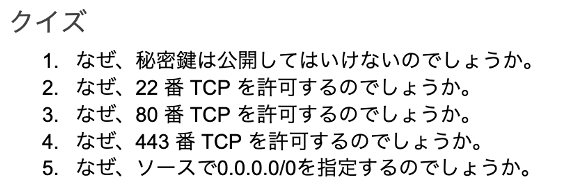
\includegraphics[width=140mm]{./img/question.png}
\caption{資料内の設問}
\label{fig:append_grech_config}
\end{center}
\end{figure}

ワークシートに準拠した構成だが,ワークシートにない解説も行った.GitHubにコードをアップロードするためにSSH鍵の作成方法なども紹介した.興味がある学生は,自主的に進められるようにした.また,最後の章には,PHP以外の言語での実装方法についての紹介も行った.この章では,詳細な解説は行わず,検索ワードの提示のみを行った.学生は,自身で調査することで,最終課題にスムーズに移行できるように工夫した.

\chapter{LAMP構成のアプリケーション}\label{append_lamp}
\renewcommand{\thepage}{B--\arabic{page}}

この演習ではOSのLinux, WebサーバーのApache,データベースのMySQL,プログラミング言語のPHPを組み合わせた環境であるLAMPと呼ばれる環境を構築した.図\ref{fig:lamp_kousei}にLAMPの構成を示す.AWSのEC2上に構築する.Apacheでリクエストを受け,PHPでリクエストに対する処理を行う.PHPからMySQLを操作し,データベース内のデータを操作する.

\begin{figure}[H]
\begin{center}
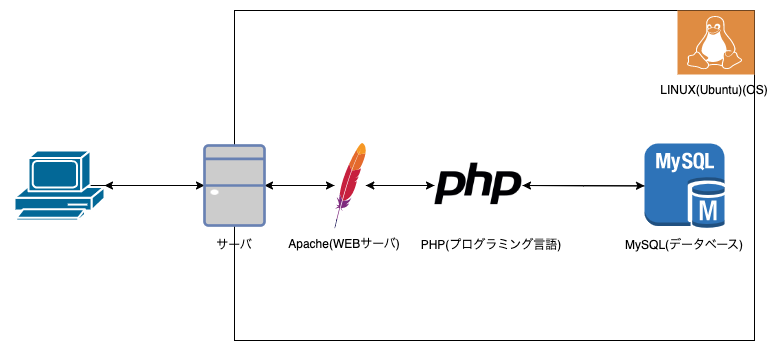
\includegraphics[width=120mm]{./img/lamp.png}
\caption{LAMP構成}
\label{fig:lamp_kousei}
\end{center}
\end{figure}

本検証のLAMP構成のアプリケーションの構築で学生が作成するPHPのコードを以下に示す.

\inputminted[breaklines,linenos,frame=lines,framesep=2mm]{php}{app.php}

単一のファイルで作成されたプログラムで,データをHTTPでPOSTからデータベースの操作までの流れを追いやすくした.付録\ref{append_worksheet}で述べた資料内でソースコードの簡単な解説を行い,PHPの記法については学生自身で調べるように指示した.

\chapter{サーバ構築支援ツール}\label{append_tool}
\renewcommand{\thepage}{C--\arabic{page}}

本研究のLAMP環境構築の演習で用いたサーバ演習構築ツール について述べる.本演習では,演習によって構築する環境に学生ごとに差異はなく,全ての学生が同じ環境を構築する.本ツールは,教員やスチューデントアシスタントが問題把握しやすくする目的や,学生自身で問題を特定できるように支援する目的のために作成した.

\begin{figure}[H]
\begin{center}
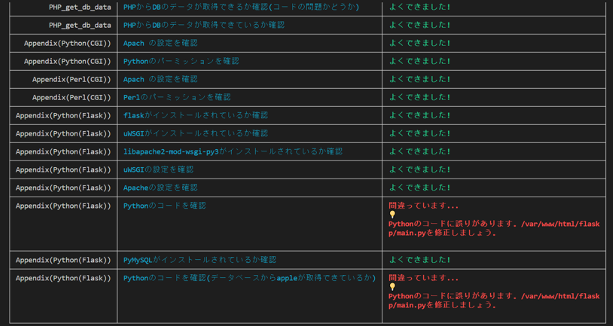
\includegraphics[width=140mm]{./img/grech.png}
\caption{サーバ演習テストツール}
\label{fig:append_grech}
\end{center}
\end{figure}


このツールの特徴は,問題に対してサーバ構築演習者に原因の解決策を提示することができることが特徴である.以下の図21に解決策をツールが行っている様子を示す.緑で示されたチェック項目は適切な設定ができている項目である.赤文字で示された項目は,誤った設定や,教員が想定していない挙動を示している項目である.テスト内容や粒度は教員が自由に作成することができる.テストの内容はYAMLで定義することができ,簡単に編集することができる.また,演習者ごとに異なる設定,例えば,データベースのパスワードなどは演習者ごとに設定ができるようにした.

\begin{figure}[H]
\begin{center}
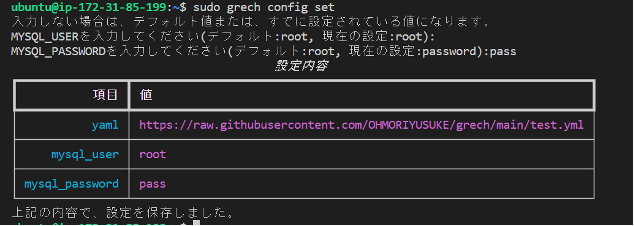
\includegraphics[width=140mm]{./img/grech_config.png}
\caption{演習者ごとに異なる設定}
\label{fig:append_grech_config}
\end{center}
\end{figure}

テスト項目が記載されたYAMLファイルはインタネット上で公開することで,演習開始後にテスト内容を変更しても,演習者の環境に即時反映させることができる.

\vskip\baselineskip

以下に示したコードがYAMLで定義されたテストの例である.

\inputminted[breaklines,linenos,frame=lines,framesep=2mm]{yaml}{test.yml}

コマンドを実行し,出力された結果が正規表現にマッチしなかった場合は想定されていない設定や挙動として処理され,演習者に改善案の提示を行う.

\vskip\baselineskip

\ref{fig:append_grech_config}で行った演習者ごとの設定やYAMLで定義されたコマンドがどのように実行されているのかを演習自身で確認することができる.図\ref{fig:append_grech_debug}に実行しているコマンドが出力されている様子を示す.

\begin{figure}[H]
\begin{center}
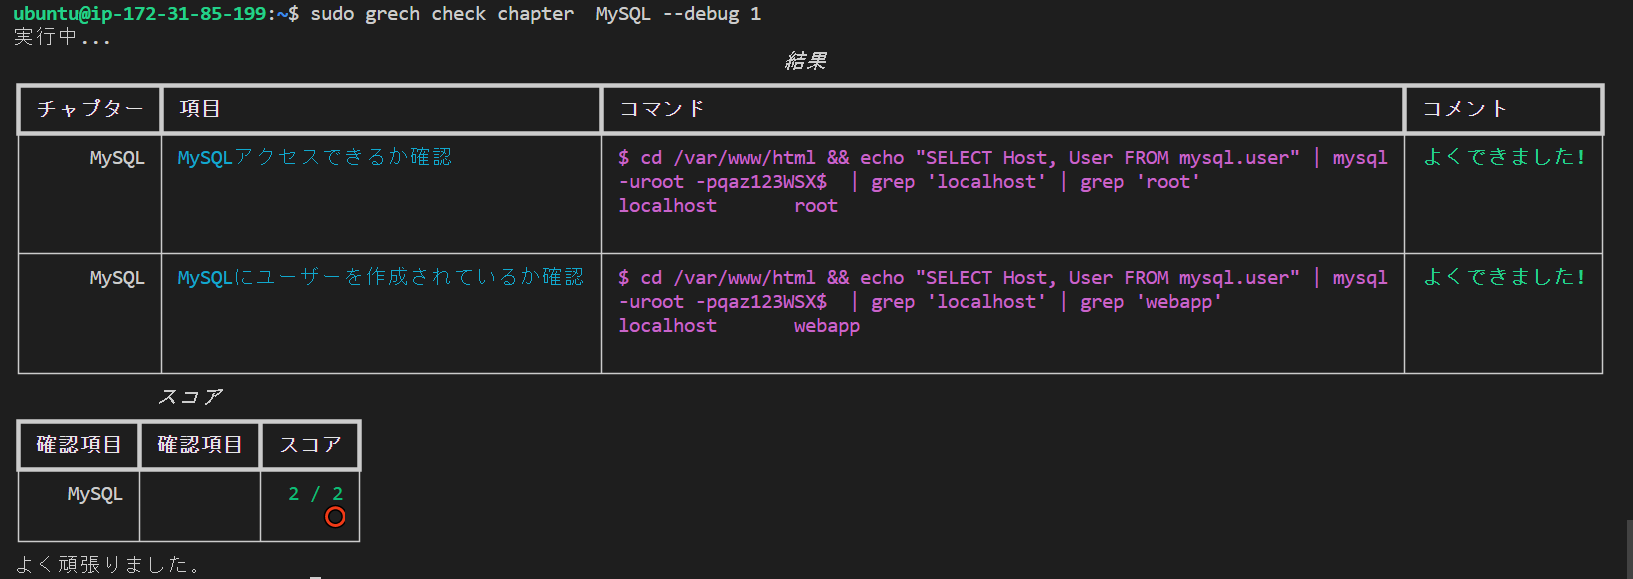
\includegraphics[width=140mm]{./img/grech_debug.png}
\caption{サーバ演習テストツール(デバッグモード)}
\label{fig:append_grech_debug}
\end{center}
\end{figure}

演習者はどのようなコマンドを実行することでツールがテストを行っているのかを確認することができる.これにより,演習者自信もコマンドを確認し,ツールを用いずに課題のデバッグを行うように促す.

\chapter{興味,関心の多さと取り組みの多さの関係についてのアンケート}\label{append_interview}
\renewcommand{\thepage}{D--\arabic{page}}

興味,関心の多さと取り組みの多さの関係について調査したアンケートの質問と回答項目について示す.

\section{興味,関心についての設問}

\paragraph{質問文}
「現在、あなたが興味を持っている分野はなんですか(複数回答可)。」

\paragraph{回答項目}
\begin{itemize}
\item プログラミング言語(授業で使ったことがあるもの、例: C、Java、Python)
\item プログラミング言語(授業で扱ってないもの、例: Go、Rust、Zig、R、C#、Kotlin)
\item システム開発(受託開発)
\item システム開発(自社開発)
\item システム開発(ネットワークやOSなど基盤システム寄り)
\item システム構築(ネットワーク)
\item システム構築(サーバ,物理的な実体あり)
\item システム構築(クラウド)
\item システム構築(営業)
\item オープンソース
\item ネットワーク構築
\item ネットワーク運用
\item 通信(光ファイバーによる通信など、有線)
\item 通信(LTE、5G、6Gなど、無線)
\item 通信(営業)
\item 機械学習(データを用いて予想をしたい)
\item 機械学習(営業)
\item 機械学習(アルゴリズム開発)
\item 人工知能(本家本元;そもそも脳の動作のしくみをしりたい)
\item サイバーセキュリティ
\item サイバーセキュリティ(営業)
\item プロジェクトマネージメント職
\end{itemize}

\section{取り組みの多さについての設問}

\paragraph{質問文}
「現在までに取り組んできたことについて教えてください。(※授業外での取り組みについて回答してください)(複数回答可)」

\paragraph{回答項目}
\begin{itemize}
\item 自分のソフトウエアを公開したことがある
\item オープンデータの作成に協力したことがある
\item patch を送ったことがある
\item pull request を送ったことがある
\item issue を立てたことがある
\item ブログにOSSの解説記事を書いたことがある
\item ドキュメントを翻訳したことがある
\item qiita や zenn などの技術ブログを書いたことがある
\item teratail や stackoverflow などで質問や回答をしたことがある
\item OSS ソフトウェアのドキュメントをまとめたことがある
\item 技術イベントで発表したことがある(LT も含む)
\item 技術イベントに視聴者として参加したことがある
\item 登壇者に質問をしたことがある
\end{itemize}

\chapter{インタビューの結果}\label{append_interview}
\renewcommand{\thepage}{E--\arabic{page}}

インタビューの詳細について述べる.インタビュー調査は1対1の対面方式で行い,その内容は音声で記録した.

\section{1人目}

\subsection{アンケートの結果}

「ワークシートが順調に進まなかった」と回答した学生の中で最も取り組んだことが多く,これから取り組んでみたいことも最も多い学生である.演習前から自信もあった学生である.
アンケートのARCSモデルの「興味」の結果は変化なし,「関連性」の結果は減少,「自信」の結果は減少している.

\subsection{インタビューの結果}

\subsubsection{演習に関する自信について}

\begin{itemize}
\item 「LAMP環境の構築は一度苦戦した点があったが,その他は苦戦していなかった.進めることはできたが,納得しながら進めることが大変で,苦戦した.」
\item 「コマンドプロンプトを見ながら演習を行うことについては,自身の興味で以前からコマンドラインテキストエディタを用いたコーデイングを行っていた.知らないものを自主的に使うことに抵抗はない.」
\end{itemize}

\subsubsection{最終課題について}

\begin{itemize}
\item 「当初思っていた入退室管理アプリはできそうだと回答した.実際にGo言語のコードを見て,このサンプルを使えばできそう.これから試す.Go言語は書いたことがない.」
\end{itemize}

\subsubsection{達成感,楽しさ,満足感について}

\begin{itemize}
\item 「演習課題については,順調に進むと楽しいと感じる.できることで達成感を感じる.」
\end{itemize}

\subsubsection{今まで取り組んできたこと}

\begin{itemize}
\item 「GitHub では他の講義の最終課題で作成したLine Botを公開している.公開してもあまり見られないだろうと思い公開してみた.」
\item 「プロメンでは,周囲の学生から影響をうけモチベーションは高まったが,できる人をみるとやる気がなくなることもあった.できる人がどんどん進めてくれる.知り合いが多いので参加した.参加するのに抵抗はなかった.」
\item 「技育展は,知人が就活で話していて知った.プロメンとは関係がない知人から知った.」
\item 「技育展に視聴参加した.全く知らない技術の話を聞いて,興味をもったが,視聴後に少し調べてみたが,詳しく調べることはなかった.調べてみたが難しかった.」
\end{itemize}

\subsubsection{これから取り組みたいこと}

\begin{itemize}
\item 「プロメンで取り組んでいたことに今も興味があるかについては,プロメンが終わった今ではプロメンで取り組んでいた内容に興味はない.現在は,大学に入学して少し学び挫折したJavaScriptを学び直したい.システム開発を行いたい.」
\item 「技術ブログを書きたいと回答.知識をまとめるために書きたいと話した.」
\item 「視聴することや,自分だけで完結することは気軽に参加,挑戦できる.」
\item 「イベントの存在をしれれば参加したいと回答した.しかし,他者と協働で行うイベントは,知り合い同士で取り組めない場合は参加することは難しいと回答した.現在は,参加したいイベントはない.」
\end{itemize}


\section{2人目}

\subsection{アンケートの結果}

「ワークシートが順調に進まなかった」と回答した学生の中で最も取り興味あることが多く,これ取り組みたいこと,取り組んだことはそれぞれ1つである.アンケートのARCSモデルの「興味」の結果は向上,「関連性」の結果は変化なし,「自信」の結果は変化なしである.

\subsection{インタビューの結果}

\subsubsection{演習に関する自信について}

\begin{itemize}
\item 「演習前に思っていたより簡単だった.」
\item 「資料を見逃しなく読むことで詰まることはあまりなかった.」
\item 「資料を見てできることが多かった.一方で,資料に書かれていないところで苦戦することがあった.資料に書かれていないことをやることは難しい.また,わからないことを調べて見つからないとストレスに感じる.最初から教えて欲しい.」
\item 「最終課題で発展的なことを求めるのであれば,発展的な内容についても資料で解説してほしい.」
\item 「わからないところが出てきた時は検索してから質問している.質問して返ってきたコメントについても調べている時にすでにみた情報であることもある.」
\end{itemize}

\subsubsection{最終課題について}

\begin{itemize}
\item 「最終課題は,技術ブログの記事を参考にして作った.当初思っていたより進んでないが,半分は進んだ.一部の機能は完成している.もっといいものを作りたいから満足していない.」
\item 「Dockerも使いたかったが,調べてもうまくいかず,エラーが解決できそうになく諦めた.Dockerも使いたかった.」
\end{itemize}

\subsubsection{達成感,楽しさ,満足感について}

\begin{itemize}
\item 「努力して(たくさん調査して苦戦して)やっとできたとしても達成感や満足感の向上に繋がることはない.」
\item 「LAMP編で作ったアプリが簡素で満足感がなかった.WEBのデザインやアプリの機能が質素である.」
\item 「アプリが質素だったから,自分で改善,改造はしていない.課題ではなかったためやらなかった.」
\end{itemize}

\subsubsection{今まで取り組んできたこと}

\begin{itemize}
\item 「興味について,今はセキュリティーに興味がある.」
\item 「就職活動のため,三年夏のインターンシップに参加してから,セキュリティミニキャンプに参加して,資格や座学で学ぶことも楽しいが,手を動かして学ぶことも重要だと思うようになった.」
\item 「外部のイベントでは,丁寧に教えてもらえる環境でないと手を動かして学ぶことは難しい.」
\item 「他大学の学生やさまざまな人と関わることは楽しいと思うようになった.知らないことを知ることができ,刺激がもらえる.」
\item 「プロメンでも活動していたが,学内や就活で有利になれると思ったから参加した.やりたいことができて満足した.プロメンで活動した内容については,今も自主的に学んでいるわけではない.」
\end{itemize}

\subsubsection{これから取り組みたいこと}

\begin{itemize}
\item 「セキュリティについて勉強したい.」
\end{itemize}


\section{3人目}

\subsection{アンケートの結果}

「ワークシートが順調に進んだ」と回答した学生の中で取り組んでみたいことは2つ,取り組んできたことは2つである.アンケートのARCSモデルの「興味」の結果は向上,「関連性」の結果は減少,「自信」の結果は変化なしである.

\subsection{インタビューの結果}

\subsubsection{演習に関する自信について}

\begin{itemize}
\item 「Raspberry Piなどに触れていた.ファイルサーバを建てたことがある.」
\item 「Apacheについては,以前, Raspberry PiでApacheを使ったことがあったので,自信があった.」
\item 「MySQLについては,実際に操作して構築した経験がなかったので自信がなかった.」
\item 「LAMPの構築を行ったことで,データベースについて理解が深まり,PHPで実装したデータベースとの連携をPythonでもできそうだと感じた.」
\end{itemize}

\subsubsection{最終課題について}

\begin{itemize}
\item 「最終課題は,DockerやAmazon Auroraを使いたいと思っていて,導入を進めている.アカウント登録などを行い,実際に手を動かしている.」
\item 「後半の課題は,前半の知識が生きた.前半の演習があったから後半ができていると思う.」
\item 「後半はPythonを使っているが,プロメンなどでPythonを使ったことがあるためPythonを選んだ.すでに,Pythonの実装は終わっている.」
\item 「Amazon AuroraやDockerに挑戦している.アドベントカレンダーに合わせてPythonの実装が終わったため,これらに挑戦している.」
\end{itemize}

\subsubsection{達成感,楽しさ,満足感について}

\begin{itemize}
\item 「何事でも,理解が浅いところを自分で深めたくなる.LAMP編では,コマンドの意味などを調べた.プロメンでは,Pythonのライブラリの内部実装などについて調べた.」
\item 「自身で調べながらやった方が達成感はある.最初の興味が湧くきっかけは先生の発言から理解が浅いと思うことを調べていく過程で興味を持つ.」
\end{itemize}

\subsubsection{今まで取り組んできたこと}

\begin{itemize}
\item 「Qiitaは講義内で紹介され,学生でも自由に書いていいと言われ,安心して記事を書くことができた.」
\item 「大学で案内された大学外のハッカソンに友人と参加した.1人だったら参加しなかった.」
\item 「プロメンで活動した.プロメンに参加した理由は,周囲から楽しいと聞いたため参加した.」
\item 「プロメンであまり教えてもらえない中,自身で調べながら開発できたのは,使命感や期待されていることを感じられてから頑張れた.」
\item 「大学外のハッカソンよりプロメンの方が印象に残っている.プロメンでは長期的な活動で,友人ができた.また,長期的な期待されて開発を行えた.」
\end{itemize}

\subsubsection{これから取り組みたいこと}

\begin{itemize}
\item 「Javaの勉強をしたい.講義でデータベースと連携したシステムを開発して勉強したが,理解ができていない気がするため.」
\item 「講義で勉強会の参加を促されたが,具体的なイベント名まで言われなかったので参加しなかった.参加することに不安がある.友人と参加したい.」
\item 「先生から参加しても大丈夫のような具体的な助言があれば参加したい.」
\item 「対面でのイベントに参加したい.」
\item 「学内のアルバイトでデータサイエンスについて取り組んでいるため,プロメンでの知識が役立っており満足感がある.アルバイトは,プロメンの活動内で募集があった.」
\end{itemize}


\section{4人目}

\subsection{アンケートの結果}

「ワークシートが順調に進んだ」と回答した学生の中で取り組んでみたいことは3つ,取り組んできたことは1つである.アンケートのARCSモデルの「興味」の結果は向上,「関連性」の結果は向上,「自信」の向上である.GitHub Issuesでエラーログのみやターミナルのスクリーンショットを投稿していた学生.

\subsection{インタビューの結果}

\subsubsection{演習に関する自信について}

\begin{itemize}
\item 「資料のみを読んで順調に進めることができた.」
\item 「資料通りにうまくいかず,エラーでしばらく詰まった.とても苦痛だった.」
\item 「演習時間外に問題の解決策について,GitHub Issuesでコメントをもらい,問題が解決できた.」
\item 「LAMP編での演習だけでは,最終課題に取り組むには不十分だった.」
\end{itemize}

\subsubsection{最終課題について}

\begin{itemize}
\item 「全く進んでいない.」
\item 「取り組みたいことがない」
\item 「LAMP編で学んだ知識では最終課題で自由に構築することはとても難しい.」
\item 「発展的な内容についても詳しく教えて欲しい.自分で調査して学ぶことは難しい.」
\item 「他の授業での自由課題でJavaのアプリを作ったが,調べて開発することができず完成させられなかった.」
\item 「自分では満足できるものを作れないので,チームで取り組みたい.」
\end{itemize}

\subsubsection{達成感,楽しさ,満足感について}

\begin{itemize}
\item 「自身で調査して解決できたとしても,達成感は感じない.」
\item 「問題の解決にかけた時間や,問題の難易度に関わらず,問題解決ができた時に達成感を感じる.簡単な問題をたくさん解決させた方が達成感を感じる.」
\end{itemize}

\subsubsection{今まで取り組んできたこと}

\begin{itemize}
\item 「プロメンは参加していない.サークル活動や部活動も行っていない.」
\item 「課外活動も取り組んでいない.」
\item 「大学の成績に関係がないので課外活動はあまりしない.」
\end{itemize}

\subsubsection{これから取り組みたいこと}

\begin{itemize}
\item 「ゲーム開発をしたいと思っているが,実際に取り組んだことはない.一人だとやらないが,チームで開発ができればやってみたいと思っている.しかし,ゲーム開発のサークルやプロメンに参加することは抵抗がある.講義時間外に拘束されることが不満である.」
\item 「プロメンやサークルでは,丁寧に物事を教えてもらえず,自身の能力を向上させることができない.個人の努力が求められる.」
\item 「丁寧に教えてもらえる有料会員制のプログラミングコミュニティーに参加したいが,お金がない.」
\end{itemize}


\section{インタビュー内の単語}

インタビューで学生がどのようなことを考えながら演習に取り組んでいたのか,どのような課外活動での取り組みをしてきたのか調査した.インタビューの中で出てきた単語について述べる.

\subsection{Go言語}

プログラミング言語.本学の講義でGo言語を扱う講義はない.本演習内で紹介した.

\subsection{技育展}

株式会社サポーターズによって行われているエンジニアを目指す学生のためのピッチコンテストである.本学で参加を進めている活動ではない.

\subsection{Line Bot, Java}

本学の講義で,Javaを学び,最後の課題としてLine Botを用いて実践的なアプリケーションの開発を行う.この課題では,学生自身で作りたいアプリケーションを決め,自由に開発する.

\subsection{Python}

プログラミング言語.本学の講義で機械学習について学ぶ際に用いる.

\subsection{Raspberry Pi, Amazon Aurora, Docker}

Raspberry Piはマイクロコンピュータである. Amazon AuroraはAWSが提供するデータベースである.Dockerはコンテナ型のアプリケーション実行環境である.CTFは,情報セキュリティの分野のコンテストである.いずれも,本学の講義で扱わない.

\subsection{セキュリティミニキャンプ}

情報セキュリティ分野に関心がある学生が短期間で情報セキュリティについて学ぶでイベントである.本学が行なっている課外活動ではない.

\subsection{プロメン}

プロジェクトメンバーの略である.本学の課外活動として,学生が主体的にITで課題の解決に取り組む活動である.

\subsection{アドベントカレンダー, Qiita}

クリスマスまでの日数をカウントダウンするアドベントカレンダーの慣習にもとづいて毎年12月1日から25日までの期間限定で開催される記事投稿イベントである. エンジニアに関する知識を記録・共有するためのサービスのQiitaでも開催されている.本講義内で,アドベントカレンダーに記事を書くこと学生に勧めた.

\end{document}